
\documentclass[hidelinks,12pt]{article}
\usepackage{lastpage}
\usepackage{fancyhdr}
\fancyfoot{}
\cfoot{\thepage{}~of~\pageref{LastPage}}
\usepackage{caption}
\usepackage[pdftex]{graphicx}
\usepackage{epstopdf}
\usepackage{mathtools}
\usepackage{amsfonts}
\usepackage{amsmath}
\usepackage{amstext}
\usepackage{amsthm}
\usepackage{enumerate}
\usepackage{amssymb}
\usepackage{breqn}
\usepackage{xr-hyper}
\usepackage{hyperref}
\usepackage{bigints}
\usepackage{color}
%\usepackage{parskip}
\usepackage[letterpaper]{geometry}
\usepackage{geometry}
\usepackage[T1]{fontenc}
\usepackage{graphicx}
\usepackage{multirow}
\usepackage{setspace}
\usepackage{keyval}
\usepackage{ifthen}
%\usepackage[american]{babel}
\usepackage{etoolbox}
\usepackage[all]{nowidow}
\usepackage[utf8]{inputenc}
\usepackage{csquotes}
\usepackage{comment}
\usepackage{placeins}
\usepackage{upgreek}
%\usepackage{natbib}
\usepackage{array}
\usepackage{adjustbox}
\usepackage[demo,abs]{overpic}
\usepackage{booktabs}

\definecolor{cadmiumgreen}{rgb}{0.0, 0.42, 0.24}
%% TO CONVERT TO TIMES NEW ROMAN
%\usepackage{mathptmx}
% convert table numering to roman
%\renewcommand*\thetable{\Roman{table}}

\usepackage[backend = biber, authordate, uniquename=false, uniquelist=false, url = false, doi=false, isbn=false]{biblatex-chicago}
\externaldocument{bpw_water_paper_appendix}

\addbibresource{bpw_water.bib}


\geometry{
top = 1in,            % <-- you want to adjust this
inner = 1in,
outer = 1in,
bottom = 1in,
%headheight = 3ex,       % <-- and this
%headsep = 2ex,          % <-- and this
}

\title{\vspace{-10mm} {Groundwater, energy, and crop choice}
}
\date{\today\\ \vspace{0.3cm} %\textsc{Preliminary and Incomplete \\ Not for citation or circulation}
}
\author{
Fiona Burlig, Louis Preonas, and Matt Woerman\thanks{\scriptsize Burlig: University of Chicago Harris School of Public Policy and NBER. Keller Center, 1307 E. 60th Street, Chicago, IL 60637. Email: \url{burlig@uchicago.edu}. Preonas: Department of Agricultural and Resource Economics, University of Maryland. 2200 Symons Hall, 7998 Regents Drive, College Park, MD 20742. Email: \url{lpreonas@umd.edu}. Woerman: Department of Resource Economics, University of Massachusetts Amherst. Stockbridge Hall, 80 Campus Center Way, Amherst, MA 01003. Email: \url{mwoerman@umass.edu}. 
%
We thank Nick Hagerty for graciously sharing data with us, and thank Amy Ando, Andrew Ayers, Maximilian Auffhammer, Kathy Baylis, Ellen Bruno, Karen Clay, Michael Greenstone, Koichiro Ito, Katrina Jessoe, Erik Lichtenberg, Dave McLaughlin, Kyle Meng, Mar Reguant, Paul Scott, Joe Shapiro, Andrew Stevens, Catherine Wolfram, and seminar participants at UC Energy Camp, Mississippi State, UC Davis, University of Illinois, ITAM, HKUST, University of Chicago, USC, the ASSA Annual Meetings, the AERE Summer Conference, the WEAI annual meetings, and UC Berkeley's POWER Conference for helpful comments and suggestions.
%
Chinmay Lohani, Anna Schmidt, Chen Sui, Yixin Sun, and Xinyi Wang provided excellent research assistance.
%
Karen Notsund provided invaluable support in obtaining data. 
%
We received generous funding in support of this project from the Giannini Foundation of Agricultural Economics, and the Sloan Foundation (via the E2e Project), and the Becker Friedman Institute for Economics.
%
All remaining errors are our own.}}
\begin{document}

\setlength{\parindent}{0.9cm}
\maketitle
\thispagestyle{empty}
\normalsize
%\vspace{-2mm}
%\thispagestyle{empty}
\begin{abstract}
%\vspace{-5mm} 
%
% Abstract

\noindent
Groundwater is a key resource for agricultural production globally. Both increasingly rapid drawdowns of aquifers as well the policies intended to increase aquifer sustainability increase costs to agricultural producers, with unknown consequences. In this paper, we provide the first large-scale empirical estimates of how farmers respond to changes in groundwater costs in one of the world's most valuable agricultural areas: California. To do this, we assemble a novel dataset that combines (i) detailed restricted-access microdata on farmers' electricity consumption, (ii) rich data from technical audits of these farmers' pump efficiencies, (iii) measurements of groundwater depths in California aquifers, and (iv) satellite-derived measures of crop cover. For identification, we leverage exogenous variation in the price of electricity, a key marginal input into the groundwater production function. We find that farmers are very price responsive: we estimate large price elasticities of demand for electricity ($-1.17$) and groundwater ($-1.12$). We demonstrate that crop switching and fallowing are the main channel through which farmers respond to increases in groundwater costs. Using a discrete choice model, we estimate that a counterfactual \$10 per-acre-foot groundwater tax---approximately the price increase required to meet California's sustainability targets---would lead farmers to reallocate 8 percent of cropland, with increases in fallowing and high-value fruit and nut perennials, and decreases in annual crops and low-value perennials. 
 %We find evidence that crop switching and fallowing is the primary mechanism behind these large elasticity estimates. {\color{magenta}Our results imply that a moderate groundwater tax of \$10 per acre-foot would cause farmers to reallocate nearly 8\% of cropland to a different crop type.} These results suggest that groundwater management policy may have important impacts on the markets for agricultural products.
%
%We then {\color{magenta}investigate possible mechanisms and find empirical evidence that the primary mechanism for these large elasticities is crop switching and fallowing in response to increased prices for electricity and groundwater.}
%{\color{blue}test two main mechanisms behind this large elasticity: substitution between groundwater and surface water, and crop switching. We find [xxx].  }\\
\\



\noindent \textbf{Keywords:} groundwater, agriculture, electricity \\
\noindent \textbf{JEL Codes:} Q15, Q25, Q41 \\
 

\end{abstract}
\vspace{5mm}

\newpage
\clearpage
\setcounter{page}{1}
\begin{refsection}
\begin{spacing}{1.5} {

\section{Introduction}
\label{sec:intro}
%
% INTRO 
%
Groundwater is an essential input into agricultural production, responsible for supplying water to 38 percent of irrigated acres worldwide (\textcite{siebert2010}). Recent scientific evidence documents rapid drawdowns of global aquifers, with key agricultural areas seeing their water tables fall by over 4 cm per year.\footnote{\url{https://www.nytimes.com/interactive/2019/08/06/climate/world-water-stress.html}} Given that global climate change is projected to increase the frequency and severity of droughts (\textcite{famiglietti2014}), governments will face a greater urgency to enact policies to manage common-pool groundwater resources. For agricultural producers who rely on groundwater for irrigation, both groundwater scarcity itself and groundwater management policies increase the costs of growing crops.

In this paper, we generate novel empirical estimates of farmers' response to changes in groundwater pumping costs in California, one of the world's most valuable agricultural regions. California produces 18 percent of total U.S.\ crop value, and its farmers rely heavily on groundwater for irrigation. Despite rapidly declining aquifer levels and a series of severe droughts, most California farmers face no meaningful restrictions on groundwater extraction. 
%remains largely unregulated in California, and most farmers face no meaningful restrictions on pumping. 
The state is currently implementing the Sustainable Groundwater Management Act (SGMA), California's first legislation governing groundwater use at scale. %This underscores the importance in predicting both the extent to which farmers will respond to new pumping regulations, and their means of adapting to higher irrigation costs.
The effectiveness and economic consequences of any such groundwater regulation depend on both the extent to which farmers will respond to new pumping regulations and their means of adapting to higher irrigation costs.

We begin by estimating the price elasticity of demand for agricultural groundwater. %We use existing work for (1), including (\textcite{sunding2010}).\footnote{In this draft, we make simplifying assumptions for these hydrological estimates. Future work will expand this to include more realistic hydrological assumptions.} 
%Despite the importance of groundwater as an agricultural input, e
Estimating this elasticity has historically proven difficult, in large  part because groundwater is typically neither priced nor measured. 
We overcome these challenges by leveraging the fact that electricity is the main variable input in groundwater extraction. Using data on electricity prices and quantities, along with farm-specific mappings from energy inputs to groundwater extraction volumes, we are able to construct measures of groundwater prices and quantities. We assemble a novel dataset that combines (i) confidential electricity consumption data for all agricultural customers served by Pacific Gas \& Electric (PGE), California's largest electric utility; (ii) technical pump efficiency audits for nearly 12,000 groundwater extraction points; and (iii) publicly available groundwater measurements across space and time, for all major California aquifers.%\footnote{\color{red} I wanted to hold off on the crop types for a bit, since they aren't part of the elasticity estimates} 
%; and (iv) satellite-derived crop type measurements.

Using exogenous variation in PGE's electricity tariff schedules, we causally identify demand elasticities for both electricity and groundwater. We estimate farmers' price elasticity of demand for electricity to be $-1.17$, which is much more elastic than prior estimates of electricity demand in the residential and commercial/industrial sectors. For groundwater, we estimate a demand elasticity of $-1.12$. This is much more elastic that previous estimates from the literature on agricultural groundwater demand. Both elasticity estimates are robust to a variety of sensitivities, and together imply that California's forthcoming groundwater management efforts have the potential to yield the substantial reductions in extraction necessary to meet the state's sustainability goals.


Given these large elasticities, a natural question is: \emph{how} are farmers reducing their water use in response to increases in groundwater costs? We consider four potential mechanisms that farmers may be engaging in: (i) applying less water to existing crops; (ii) changing irrigation efficiency; (iii) switching water sources; and (iv) switching crops or fallowing. We present empirical evidence against (i): farmers do not appear to adjust water consumption in response to large short-run fluctuations in price. We can also rule out (ii): we estimate quantitatively similar groundwater elasticities in the short windows around pump tests, where major changes in pumping capital are highly unlikely. We then develop a stylized model of farm crop choice and irrigation costs to provide theoretical guidance on (iii) and (iv). This model reveals that (iii) is only likely at extremely high groundwater pumping costs---which we rarely observe in our data---at which point farmers may substitute groundwater for water purchased on the open market (\textcite{hagerty2018}).

This leaves crop switching as the leading candidate mechanism driving farmers' groundwater large demand response. We conduct several empirical tests to provide evidence in support of this crop switching mechanism. We estimate annual elasticities that are similar to our monthly elasticities, suggesting that farmers are not arbitraging water sources within a growing season. We find that these annual elasticities can be decomposed into substantial intensive- and extensive-margin responses to increasing groundwater costs, consistent with farmers switching to less-water-intensive crops and fallowing land. 

Building on these results, we estimate a discrete choice model of farmers' cropping decisions to directly quantify the causal effect of groundwater costs on land use. Using a multinomial probit model, identified using exogenous variation in PGE's electricity tariffs, we find that increases in groundwater costs reallocate cropland across four broad crop types. A 10 percent increase in the cost of groundwater causes farmers to increase the proportion of land in fruit and nut perennials by 1.0 percentage point, increase fallowed land by 0.4 percentage points (almost identical to our extensive-margin semi-elasticity), decrease land in annuals by 0.9 percentage points and reduce land in other perennials by 0.5 percentage points. Because we use a static discrete choice model, these are likely underestimates of the true impacts of increasing groundwater costs on crop reallocation (\textcite{scott2013}). %Dynamics are likely important in this context, however, meaning that these static estimates understate true switching. In ongoing work, we are adapting the dynamic discrete choice framework developed by \textcite{scott2013} to our context, in order to incorporate state dependence in crop choice.


Finally, we simulate how cropland would be reallocated in response to a counterfactual groundwater tax---a regulation that could internalize open-access externalities and achieve sustainable levels of groundwater extraction.\footnote{The water economics literature typically cites two main externalities associated with groundwater extraction (\textcite{provencher1993}). The first is the ``stock externality'', which arises from the finite nature of non-renewable groundwater stocks, driving farmers to collectively extract faster than the social planner's optimal extraction path. The second is the ``pumping cost'' externality: when a farmer extracts an acre-foot of groundwater from an aquifer, the water level falls, increasing pumping costs for other (nearby) users. Recently, other potential externalities such as air quality issues associated with soil drying and land subsidence have been raised as well.}  Under SGMA, California will require high-use basins to reduce extraction by between 20 and 50 percent (\textcite{bruno2019}). We find that a \$10 per acre-foot tax on groundwater, representing approximately a 25 percent increase in pumping costs, would result in a 27 percent reduction in groundwater extraction, near the low end of this targeted curtailment range. We estimate that this same tax would lead farmers to reallocate nearly 8 percent of cropland to a different crop type. While the level of the efficient Pigouvian groundwater tax remains unknown, if the true externality is around \$10 per acre-foot, our results imply that that 8 percent of total cropland in California is currently misallocated from its socially optimal use.


This paper makes three main academic contributions. First, we provide the first large-scale empirical estimates of the impact of groundwater pricing on crop choice in one of the most valuable agricultural regions of the world: California. We demonstrate that, as groundwater extraction costs rise, farmers respond by increasing fallowing, shifting into fruit/nut perennials (among the highest-revenue crops per acre-foot of water), and shifting out of low-value perennials and annual crops. These results have important implications for agricultural markets, as California is a monopoly producer of many crops that may become less prevalent under groundwater regulation. They also contribute estimates from an understudied sector to the broader literature on the impacts of environmental regulation.



Second, to quantify the impacts of groundwater cost increases on land use, we begin by contributing novel estimates of the price elasticity of electricity demand in agriculture---a major, but heretofore overlooked, electricity end-use sector. While many studies estimate the relationship between electricity prices and consumption in the residential sector (\textcite{alberini2011}; \textcite{fell2014}; \textcite{ito2014}; \textcite{deryugina2018}), far fewer have focused on commercial/industrial electricity consumption (\textcite{paul2009}; \textcite{jessoe2015}; \textcite{blonz2016}). To the best of our knowledge, there exists no comparable study estimating the price elasticity of electricity demand in the agricultural sector. By leveraging microdata for thousands of agricultural consumers across PGE's service territory, along with plausibly exogenous changes in farmers' marginal electricity prices, we identify California farmers as unusually elastic electricity consumers (a central elasticity estimate of $-1.17$), with potential implications for agricultural electricity pricing. 

Third, we leverage the central role of electricity use in groundwater extraction to estimate the elasticity of groundwater demand for California farmers---a policy-relevant elasticity that has proven elusive due to both data and identification challenges (\textcite{mieno2017}). Our empirical strategy overcomes many of these challenges by combining comprehensive electricity consumption data with technical audits of groundwater pumps, and by leveraging exogenous variation in electricity prices (a major component of pumping costs) to credibly identify changes in farmers' effective price of groundwater. 
Many previous studies have estimated water demand outside the agricultural sector (\textcite{hewitt1995}; \textcite{renwick2000}; \textcite{olmstead2007}), while others have focused specifically on groundwater demand in agriculture (\textcite{hendricks2012}; \textcite{pfeiffer2014}; \textcite{badiani2015}). We provide well-identified groundwater demand estimates for thousands of farms in one the most important agricultural regions in the world: California's Central Valley. We find that farmers are surprisingly elastic, with a central estimate of $-1.12$. We rule out several hypotheses about what might be driving this large elasticity, and demonstrate that crop reallocation is the major mechanism behind farmers' responses to increases in water costs.  

%Finally, we go beyond documenting that farmers are price-responsive groundwater consumers by {\color{blue} demonstrating that crop switching and fallowing is the primary mechanism by which they re-optimize in the face of rising input costs.} Our results imply that groundwater policies that raise the (effective) cost of water will likely lead to large shifts in crop choice. 

Beyond our contributions to the academic  literature, our findings have direct and immediate policy relevance for California agriculture, as SGMA goes into effect. If we extrapolate beyond our sample to all agriculture in California agriculture, our simulations suggest that the \$10 per acre-foot tax required to meet the lower end of SGMA's groundwater sustainability targets would reallocate nearly two million acres of cropland across the state. Our elasticity estimates also suggest that meeting the approximately 50 percent groundwater use reduction targets in severely overdrawn basins will require a tax greater than \$15 per acre-foot---more than 37 percent of the average cost per acre-foot we observe in our sample. 

This paper proceeds as follows. Section~\ref{sec:background} provides background on groundwater pumping, California agriculture, and energy use in farming. Sections~\ref{sec:data} and \ref{sec:empirics} describe our data and empirical strategy. Section~\ref{sec:results} presents our demand elasticity estimates. In Section~\ref{sec:mechanisms}, we explore mechanisms, and demonstrate the impacts of groundwater costs on crop switching.
Section~\ref{sec:conclusion} concludes. 


\section{Background}
\label{sec:background}
%
% BACKGORUND 
%

\subsection{Agriculture in California}
California is a key player in global agricultural production, and represented 17 percent of total U.S. crop value in 2016 (\textcite{crs2015}). California's 77,000 farms produce over 400 commodities, including close to half of all fruits, nuts, and vegetables grown in the United States. In fact, California is the sole domestic producer of many high-value crops, including almonds, artichokes, olives, and walnuts (\textcite{cdfa2011}).  

%\subsubsection{Agricultural water use}
Water is an essential input for California's agricultural production. Nearly 80 percent of the state's annual water consumption occurs in the agricultural sector, where crop irrigation is the primary end use. California has nearly 8.3 million harvested acres of cropland, 7.9 million of which are irrigated (\textcite{crs2015}). Farmers may have access to surface water and/or groundwater, and each water source is governed by a complex system of rights.\footnote{See \textcite{sawyers2007} for more details.} 


\begin{comment}
\paragraph{Surface water}
{\color{blue}
Approximately 40 percent of California's surface water is used in agriculture. 61 percent of irrigation water comes from surface sources, with groundwater making up the remaining 39 percent {\color{blue}(CA DWR 2015, cite in hagerty p 7)}. Most farms with access to surface water obtain it via irrigation districts.\footnote{Irrigation districts were established between 1860 and 1950, and their boundaries have remained essentially fixed over time. Though some individual farms do have their own water entitlements, the vast majority of these allocations belong to districts. {\color{blue} would be good to get a stat on this}.} These agricultural cooperatives divert water from large rivers and canals and distribute this water to farmers, with individual farmers receiving water proportional to their acreage within the district (\textcite{schlenker et al 2007}). 

Irrigation districts obtain water through two main sources: project contracts and water rights. Project contracts allow irrigation districts to withdraw water from state- and federally-operated canals.\footnote{There are three such water projects in California: the State Water Project, the Central Valley Project, and the Lower Colorado Project. The State Water Project is managed by the California government; the other two are federally managed.} Water rights allow irrigation districts to withdraw water from nearby rivers and streams. In California, These rights are under a prior appropriation system, meaning that rights are established by the first claimant, and held as long as water is continuously used.  

Both water rights and project contracts provide irrigation districts with fixed \emph{maximum} appropriations over time, but annual allocations can vary across years. Under drought conditions, water rights are allocated according to the age of the right. Senior rightsholders, with rights established prior to 1914, are entitled to their full allocation in all years. Junior rightsholders, with rights established in and after 1914, are ranked in order of age of the right, and allocated water until the maximum allotment has been distributed. {\color{blue} WE SHOULD TRIPLE CHECK TO MAKE SURE THIS IS ACTUALLY ACCURATE.} Project contracts also vary their allocations year by year, using an algorithm which depends only on environmental conditions. {\color{blue} something about how this works by giving you a share of your max allotment.} Information on allocations is revealed to farmers well in advance of the growing season.

For a more detailed description of surface water rights in California, see \textcite{hagerty2019}.}
\end{comment}

\paragraph{Surface water}
Approximately 40 percent of California's surface water is used in agriculture. 61 percent of irrigation water comes from surface sources, with groundwater making up the remaining 39 percent (\textcite{cdwr2015}). Surface water rights in California follow strict rules. Most farms with access to surface water obtain it via irrigation districts.\footnote{Irrigation districts were established between 1860 and 1950, and their boundaries have remained essentially fixed over time. Though some individual farms do have their own water entitlements, the vast majority of these allocations belong to districts. These agricultural cooperatives divert water from large rivers and canals and distribute this water to farmers, with individual farmers receiving water proportional to their acreage within the district (\textcite{schlenker2007}). For a more detailed description of surface water rights in California, see \textcite{hagerty2019}.} In addition to obtaining surface water from individual rights or irrigation districts, farmers have a limited ability to purchase water on the open market. However, these trades constitute only a very small share of total water deliveries, and the prices are extremely high (\textcite{hagerty2018}).


\paragraph{Groundwater}
In normal weather conditions, groundwater supplies 30 to 40 percent of all water end uses in California. However, this rises to close to 60 percent in drought years, when surface water is unusually scarce (\textcite{cdwr2014}).
By contrast to the strictly defined surface water rights, agricultural groundwater rights tend to be far more vague. The typical groundwater right in California is ``overlying,'' meaning that landowners whose property sits above an aquifer have the right to extract the underlying groundwater.\footnote{
There are also ``appropriative'' groundwater rights, for users who do not own land above the aquifer, but these rights are lower-priority than the overlying rights. Appropriative rights holders may only exercise these rights in the case of a surplus.}
The vast majority of groundwater use is unmetered, and users face no variable costs of extraction beyond the energy costs of pumping (\textcite{bruno2018}).\footnote{There are limited exceptions to this rule: a few irrigation districts impose a per-unit price on groundwater, but this is rare (\textcite{bruno2018}).} Hence, a farmer may extract as much groundwater as he chooses, conditional on owning the overlying property rights. 

Many of California's groundwater basins are ``overdrafted,'' meaning that, annually, withdrawals exceed replenishment. As of 2017, some agricultural regions were facing overdraft of 2 million acre-feet annually. This has led to a substantial decline in groundwater levels in the Central Valley, most notably in the Tulare and San Joaquin groundwater basins, which, combined, lost more than 135 million acre-feet of groundwater since 1925.\footnote{See: \url{https://www.ppic.org/publication/groundwater-in-california/}} In 2014, the state faced a severe drought, with groundwater levels reaching historic lows in many portions of the state. 21 of the state's 515 groundwater basins are considered ``critically overdrafted.''

In response to drought conditions, in September 2014, California lawmakers passed sweeping groundwater legislation. The Sustainable Groundwater Management Act (SGMA), consists of three bills, and represents  represents the first statewide regulatory scheme to mitigate over-extraction of groundwater. AB 1739 enables the California Department of Water Resources (DWR) or local groundwater sustainability agencies (GSAs) the ability to charge fees for groundwater extraction, and requires GSAs to prepare groundwater sustainability plans (GSPs). SB 1319 authorizes GSAs to implement these GSPs. SB 1168 requires that uses of groundwater be both reasonable and beneficial, and enables GSAs and the DWR to require groundwater monitoring. In addition, Proposition 1 provided \$100 million in funding to support sustainable groundwater management. SGMA represents the future of groundwater management in California. However, the GSPs will not be finalized until 2020 at the earliest, leaving farmers free to extract at will.

\subsection{Electricity for pumping}
Electricity is an essential input to groundwater pumping. The California Energy Commission reports that water use accounts for 19 percent of California's electricity consumption, and close to 8 percent of the state's energy is used on farms (\textcite{cec2005}). The state's investor-owned utilities spend nearly \$50 million annually to improve energy efficiency in the agricultural sector. This makes water use, and agricultural water use in particular, a key component of California's energy policy goals.

To estimate groundwater demand, we exploit the fact that electricity is a major determinant of pumping costs. Several previous papers have used variation in energy costs to estimate the price elasticity of groundwater demand (\textcite{hendricks2012}, \textcite{pfeiffer2014}, \textcite{badiani2015}, and \textcite{mieno2017}). However, \textcite{mieno2017} point out that these estimates may exhibit bias due to (non-classical) measurement error and/or poor identification. Furthermore, data limitations have restricted previous studies to relatively narrow geographies, which may reduce their external validity.
By contrast, our sample includes thousands of farms throughout California's Central Valley, one of the most productive agricultural regions in the world. Our data also allow us to overcome the standard measurement issues and identification challenges---via detailed technical audits that precisely characterize the electricity-to-groundwater conversion factor, and via exogenous variation in Pacific Gas \& Electric's (PGE) agricultural electricity tariffs.

%In contrast, we estimate the price elasticity of demand for agricultural groundwater throughout California's Central Valley, one of the most important agricultural regions in the world. We use a multi-step estimation process. We begin by using plausibly exogenous variation in energy pricing, both in the cross-section and over time to calculate the price elasticity of electricity consumption. We then combine this with detailed (time-varying) data on farm-specific pump characteristics and spatially explicit information on groundwater levels. With these additional data, we can estimate the price elasticity of groundwater demand with respect to (1) electricity prices, (2) groundwater levels, and finally, (3) water costs. 

\begin{comment}

\begin{itemize}

\item APEP pump tests are the other piece of this puzzle, and we can observe pump-specific conversion rates.

\end{itemize}
	
\end{comment}




\section{Data}
\label{sec:data}
%
% DATA 
%
% Normally I like empirical strategy --> data, but here I think it makes more sense to put the data first, since you kind of need to understand the electricity data before walking through the regression framework

\subsection{Electricity data}

We begin by estimating how farmers' electricity consumption responds to changes in electricity price. We use confidential customer-level electricity datasets, which PGE's data management team prepared for us under a non-disclosure agreement. These data comprise the universe of agricultural electricity consumers in PGE's service territory, and we observe each customer's monthly bills at the service account level for the years 2008--2017. We aggregate service accounts up to 108,172 unique service points (i.e.\ the physical location of an electricity meter) and construct a ``monthified'' panel of electricity consumption (in kWh) at the service point (SP) level.\footnote{
PGE's monthly bill cycles are customer-specific, and most billing periods do not line up with calendar months. We ``monthify'' billed kWh for each SP by splitting/weight-averaging multiple bills in a single calendar month, in order to create a SP by month panel. This is standard practice in the economics literature on electricity demand (e.g. \textcite{ito2014}). Most service points have a single service account at each point in time, but service accounts often turn over within a given service point.
}
We also observe several key covariates for each service point: its latitude and longitude; an indicator for accounts with solar panels on net-energy metering, which we drop from our estimation sample; and an identifier to link service point locations to physical electricity meters. Figure \ref{fig:pge_ca_map} maps all agricultural service points in our dataset.

PGE offers 23 distinct agricultural tariffs, and our billing data report the particular tariff associated with each monthly bill. Prices on each tariff are updated multiple times per year, and historic prices are publicly available, along with information on tariff-specific rules and eligibility criteria. We use these data to construct a 10-year panel of hourly volumetric (marginal) electricity prices, which we collapse to the monthly level by taking an unweighted average across hours.
%\footnote{In Appendix {\color{blue} XXX}, we explore alternative approaches to constructing prices, including using the minimum weekly (????) price rather than the monthly average price.} 
Importantly, unlike PGE's residential electricity prices, its agricultural tariffs are not tiered: a farm's marginal price does not depend its consumption. 

Variation in average volumetric price arises from several features of PGE's tariff structure. All 23 tariffs have higher marginal prices during summer months (May--October). Time-varying tariffs have higher marginal prices on weekdays, during peak hours (12--6pm), and on critical peak event days.\footnote{Critical peak pricing is a form of electricity price in which farms are offered a slightly lower electricity price throughout the year. In exchange, PGE can raise the price substantially on 15 days throughout the summer, with one or two days' notice. These event days typically occur on the hottest days of the summer. See \textcite{blonz2016} for more details on critical peak pricing. Appendix Table~\ref{tab:pge_ag_tariffs} summarizes the pricing structure for each tariff.} Fixed charges (per kW) also play an important role in offsetting marginal prices (per kWh): rates with higher marginal prices tend to have lower fixed charges, and vice versa. On top of these cross-sectional differences in tariffs pricing schemes, PGE adjusts tariffs' marginal prices differentially over time. 

PGE's 23 agricultural tariffs are divided into five mutually-exclusive categories. These five categories have strict eligibility criteria, defined both by physical pumping capital (small pumps, large pumps, or auxiliary internal combustion engines) and by type of electric meter (conventional meter, or smart meter).\footnote{Conventional meters record electricity consumption using an analog dial, whereas smart meters can digitally store the full time profile of consumption. During our sample period, PGE gradually phased out conventional meters, replacing them with smart meters capable of supporting time-varying electricity pricing.} Each of these five categories has a ``default'' tariff; other tariffs within each category are highly correlated with these default tariffs. Figure~\ref{fig:marg_price_5_default_rates} plots the five time series of default monthly average marginal prices. Our identification strategy relies on the fact that average marginal prices do not move in parallel across these five default tariffs. It also leverages the strict eligibility rules which place customers into categories. Appendix~\ref{app:pge_prices} presents more details on the full set of PGE agricultural tariffs.


%\footnote{\color{blue} Appendix Figure XXX plots a similar picture for all rates in our sample. DO WE WANT TO SAY SOMETHING ABOUT HOW CPP DAYS EXPLAIN SOME OF THIS VARIATION TOO?} {\color{magenta}Are we doing the residualized version of Figure~\ref{fig:marg_price_5_default_rates} too?} Using this tariff information, we assign each service point a monthly average marginal electricity price in \$/kWh.
 
 
 
\subsection{Pump data}

To complement our electricity data, we have rich data on agricultural groundwater pumps collected by PGE's Advanced Pumping Efficiency Program (APEP). These data include the universe of APEP-subsidized pump tests from 2011--2017, and we observe detailed measurements and technical specifications for 21,851 unique tests at 17,107 unique pump locations. Importantly, we also observe identifiers for the electricity meter associated with each pump test, which we use to match pump tests to electricity service points---thereby isolating a sample of 11,849 service points for which agricultural groundwater pumping is confirmed to be a major end-use. We restrict our empirical analysis to this 11 percent subset of agricultural service points, in order to best isolate groundwater pumpers and avoid incorporating other agricultural electricity end uses.\footnote{
Pumping is likely the only end use at matched service points, as PGE typically installs a dedicated meter for each groundwater pump. We are currently working on using satellite images to predict whether service points outside the APEP-matched sample are also groundwater pumps. We hope to incorporate these farms into future analysis, as there are likely many groundwater pumps that never received an APEP-subsidized pump test. Note that not every customer on an agricultural tariff is pumping groundwater. We restrict our sample to the APEP-matched customers in order to avoid avoid including service points with other agricultural end uses, such as operating machinery or heating greenhouses.}


Table \ref{tab:elec_summary_stats} reports summary statistics for this subset of agricultural service points (in the right column). Compared to the full set of PGE's agricultural customers, APEP-matched service points tend to consume nearly twice as much electricity and tend to pay lower marginal prices. %Only 28 percent of service points shift across tariff categories, and the vast majority of switches are triggered by PGE's smart meter rollout. 
Figure \ref{fig:pge_ca_map} reveals that APEP-matched service points are heavily concentrated in California's Central Valley and appear to be a geographically representative subset of PGE's agricultural customers.

After identifying a subset of agricultural consumers who pump groundwater, we use APEP data to characterize pump-specific groundwater production functions. 
%Groundwater extracted is Leontief in electricity (for pumps with electric motors), and 1 kWh of electricity in will yield a particular volume of groundwater out (measured in acre-feet (AF)). 
The amount of groundwater extracted is a linear function of the electricity consumed by the pump; pump characteristics and groundwater depth determine how much water (measured in acre-feet (AF)) is produced by each kWh of electricity consumed.
This kWh per AF relationship is governed by physics:
\begin{equation}
\frac{\text{kWh}}{\text{AF}} ~=~ \text{kW} \div \frac{\text{AF}}{\text{hour}} 
 ~=~ \frac{\big[\text{Lift (feet)} \big]\times \big[\text{Flow (gallon/minute)}\big]}{\big[\text{Operating pump efficiency (\%)}\big] \times \big[\text{Constant}\big]} \div \frac{\text{AF}}{\text{hour}} 
\label{eq:kwhaf_formula1}
\end{equation}
The power (kW) required to pump 1 acre-foot is directly proportional to both the vertical distance the water must travel to the surface (i.e.\ lift) and the speed at which the water travels (i.e.\ flow). It is inversely proportional to the rate at which the pump converts electric energy into the movement of water (i.e.\ operating pump efficiency). We can simplify Equation (\ref{eq:kwhaf_formula1}) by converting from gallons to acre-feet: 
\begin{equation}
\Rightarrow~~\frac{\text{kWh}}{\text{AF}} ~=~ \frac{\big[\text{Lift (feet)} \big] \times \big[\text{Constant}\big]}{\text{Operating pump efficiency (\%)}} 
\label{eq:kwhaf_formula2}
\end{equation}
For each APEP pump test, we observe measurements of kWh/AF, operating pump efficiency, flow, and lift. We also observe the standing water level, or the baseline groundwater depth in the absence of pumping. Because pumping lowers the water level at a given location, standing water levels help us more accurately calibrate how changes in aquifer depth impact lift for each pump.\footnote{
Lift is (approximately) the sum of the standing water level, drawdown (i.e., how much pump $i$ impacts its own depth), and other pump-specific factors (e.g., discharge pressure, gauge corrections, height of the pump above the surface).
Drawdown depends on rate of extraction (i.e.\ flow) and the physical properties of the substrata. Greater flow increases drawdown, as water levels fall with faster extraction. More transmissive (or porous) rock formations have lower drawdown, because water levels are able to horizontally reequilibrate  more quickly.
}


\subsection{Water data}

While a given farm's pumping technology is relatively constant in the short run, its kWh/AF conversion factor is sensitive to short-run changes in groundwater levels. In order to capture these short-run shocks in pumping costs, we use publicly available groundwater data from California's Department of Water Resources collected under the California Statewide Groundwater Elevation Monitoring (CASGEM) Program.\footnote{
These data are available from: 
\url{https://water.ca.gov/Programs/Groundwater-Management/Groundwater-Elevation-Monitoring--CASGEM}
} 
These data report depth below the surface at 16,490 unique monitoring stations during our 2008--2017 sample period, with an average of 27 measurements at each location at different points in time. We rasterize all measurements within each month (and quarter), using inverse distance weighting to interpolate a gridded two-dimensional surface of average depth at each point in space. This allows us to construct a monthly (and quarterly) panel of estimated groundwater depths at each electricity service point.

We assign each service point to a groundwater basin, using publicly available shapefiles maintained by the California Department of Water Resources.\footnote{Water basin shapefiles are available from \url{https://water.ca.gov/Programs/Groundwater-Management/Bulletin-118}. 
%Water district shapefiles are available at \url{https://data.cnra.ca.gov/dataset/water-districts}.
}
 Groundwater basins are broadly defined by stratigraphic barriers through which water does not travel horizontally. We control for annual changes in water levels that impact all farms within the same water basin. We also obtained shapefiles of irrigation districts in California from the California Department of Water Resources, the California Atlas, and the California Environmental Health Tracking Program, following \textcite{hagerty2019}. We spatially match PGE service points to these shapefiles to determine to which irrigation district (if any) each service point belongs.\footnote{In ongoing work, we are working to incorporate data on each irrigation district's water allocations for a heterogeneity analysis.} Irrigation districts (a.k.a.\ water districts) are administrative entities that govern farmers' annual allocations of surface water. Because groundwater and surface water are obvious substitutes, we non-parametrically control for annual shocks to farms' surface water allocations at the water district level. This helps to isolate variation in pumping behavior driven by variation in pumping costs, rather than variation in the availability of groundwater substitutes.
 %\footnote{
%We are currently working to incorporate additional spatial data products, including (i) shapefiles of common land units, which correspond to agricultural fields; (ii) shapefiles of parcels, which roughly correspond to farms; and (iii) the USDA Cropland Data Layer, which uses satellite imagery to classify fields by crop type. Together, these data will enable us to aggregate up from service points to farms, and to build a panel of crop choices at the farm-year level.
%}

\subsection{Groundwater prices and quantities}

We merge the above data sources to create a panel of groundwater prices and quantities at the service point by month level. To convert from electricity (kWh or \$/kWh) to groundwater (AF or \$/AF), we simply need to populate a kWh/AF conversion factor for every panel observation. We construct estimates of kWh/AF by parameterizing Equation (\ref{eq:kwhaf_formula2}) using (i) monthly (or quarterly) rasters of groundwater depths at each service point; (ii) pump-specific conversions between standing water level and lift, as calculated from APEP pump tests; and (iii) APEP-measured operating pump efficiencies. We take unweighted averages of APEP variables across multiple pumps within a single service point; we also extrapolate each service point's first pump test backwards, extrapolate its last pump test forwards, and interpolate between multiple pump tests using a triangular kernel in time. 

Table \ref{tab:water_summary_stats} reports summary statistics for this merged panel dataset. We observe 1.67 unique pump tests for the average APEP-matched service point, and APEP data reveal substantial cross-sectional variation in operating pump efficiencies and kWh/AF conversion factors. Our constructed  kWh/AF estimates tend to moderate extreme values, which compresses the right tail of measured kWh/AF (while also slightly shifting this distribution left). Interestingly, implied marginal groundwater prices exhibit far less seasonal variation than marginal electricity prices. This is because groundwater levels tend to be higher in summer months (compared to winter months), which tends to reduce (constructed) kWh/AF in months when electricity prices are highest.


%\subsection{Surface water data} We obtained shapefiles of irrigation districts in California from the California Department of Water Resources, the California Atlas, and the California Environmental Health Tracking Program, following \textcite{hagerty2019}. We spatially match PGE service points to these shapefiles to determine to which irrigation district (if any) each service point belongs.\footnote{In ongoing work, we are expanding upon this by using data on each irrigation district's water allocations in a heterogeneity analysis.}


\subsection{Agricultural data}
\paragraph{Common Land Units} 
In order to match electricity meters to cropland, we use the USDA Farm Service Agency's Common Land Unit (CLU) data. We obtained the universe of USDA CLUs in California.\footnote{In the 2008 Farm Bill, the CLU data were made restricted-access. We therefore use the 2008 CLUs for our full sample. The USDA provides more detail on CLUs here: \url{https://www.fsa.usda.gov/programs-and-services/aerial-photography/imagery-products/common-land-unit-clu/index}.} A CLU is the smallest contiguous unit of agricultural land under common land cover, land management, and ownership. We link PGE service points to CLUs via a spatial match. We also use shapefiles of tax parcels from California county assessors to aggregate CLUs ($\sim$ fields) into groups with a common owner ($\sim$ farms).\footnote{We collected tax parcel shapefiles from each county assessor's office in California. Aggregating CLUs within the same tax parcel lets us test for sensitivity to within-farm spillovers.} 

\paragraph{Cropland Data Layer} We obtain data on cropped acreage from the U.S. Department of Agriculture's (USDA) Cropland Data Layer (CDL). This 
%satellite-derived 
product provides annual information on what crop is being grown at every 30-by-30 meter pixel in the United States from 1997 to 2019. California was added to the CDL starting in 2007. The CDL is generated using satellite imagery in conjunction with a machine learning algorithm and is ground-truthed against the USDA's Farm Service Agency's farm surveys. In California during our sample period, the CDL reports 83 distinct landcover classifications. We classify these landcover categories into four broad groups: annual crops, fruit and nut perennial crops, other perennial crops, and fallowed land. The major annual crops in our sample are winter wheat, cotton, tomatoes, corn, rice, and strawberries. The major fruit and nut perennial crops are almonds, grapes, walnuts, pistachios, and oranges. The other perennials category is primarily cropped in alfalfa. The fallow category consists of land that is fallowed according to the CDL, as well as grass and pastureland.%\footnote{\color{red}Double check that things like parking lots are getting removed.}

We construct an annual panel of landcover at the CLU level based the modal CDL pixel within the CLU. If this modal crop type does not cover over 50 percent of pixels in the CLU, we label the CLU as having missing data. Using our CLU to service point concordance, we are able to assign individual service points a landcover type for each growing season.
%\footnote{In ongoing work, we are constructing additional cropping variables, including the share of land in a CLU under different crop types.} 

\subsection{Weather data}
Weather is a key input into agricultural production, which directly impacts groundwater consumption. We obtained daily temperature and precipitation rasters from the PRISM climate group, a standard source in the agriculture economics literature (see, e.g., \textcite{schlenker2009} and \textcite{burke2016}).\footnote{These data are available at \url{https://prism.oregonstate.edu/}. } Using gridded data with a 4km-by-4km resolution, we extract daily maximum temperature, minimum temperature, and precipitation at each SP location.



\section{Empirical strategy}
\label{sec:empirics}
%
% EMPIRICAL STRATEGY 
%

This section outlines our empirical strategy for estimating farmers' demand for groundwater pumping. First, we estimate price elasticities of demand for electricity, for the full sample of agricultural consumers where we can match an electricity meter to a groundwater pump. Next, we estimate price elasticities of demand for groundwater, by translating prices/quantities of electricity into prices/quantitites of water using data on (i) technical pumping production functions and (ii) groundwater depths across space and time.

\subsection{Electricity demand}\label{sec:empirics_elec}

We estimate monthly electricity demand using the following specification:
\begin{equation}
\sinh^{-1}\big(Q^{\text{elec}}_{it}\big) = \beta \log\big(P^{\text{elec}}_{it}\big) + \gamma_{i} + \delta_t + \varepsilon_{it}
\label{eq:reg_elec}
\end{equation}
The dependent variable is kWh consumed at electricity service point $i$ in month $t$, transformed using the inverse hyperbolic sine function (which closely approximates the natural log transformation but includes zero in its support).\footnote{
Since 15 percent of observations in this panel are zeroes, we apply the inverse hyperbolic sine transformation to avoid dropping months where farms consume zero kWh for groundwater pumping.
}
$P^{\text{elec}}_{it}$ is unit $i$'s marginal electricity price (in \$/kWh), averaged across all hours in month $t$. We include unit by month-of-year fixed effects ($\gamma_i$), in order to control for within-pump/month average consumption (e.g., service point $i$ in March). We also include month-of-sample fixed effects ($\delta_t$) to control for trends in both electricity prices (which rise over time) and pumping behavior. Alternative specifications include groundwater basin by year fixed effects (to control for time-varying trends in groundwater depth across basins), water district by year fixed effects (to control for annual shocks to surface water allocations), and unit-specific linear time trends.
We two-way cluster standard errors by service point and month-of-sample, which accommodates both arbitrary within-unit serial correlations and arbitrary spatial correlations with each monthly cross-section.

\subsubsection{Identification}
To identify the demand elasticity in Equation (\ref{eq:reg_elec}), we must purge any endogenous variation in unit $i$'s marginal electricity price. PGE's agricultural tariff \emph{schedules} are the outcome of statewide regulatory proceedings, and marginal prices are linear in kWh consumed.\footnote{
By contrast, PGE's residential electricity tariffs use increasing block pricing, where a household's marginal price is endogenous to its own consumption (\textcite{ito2014}). Linear marginal prices simplify 
our estimation of agricultural electricity demand, because farm $i$'s marginal price is determined \emph{solely} by its tariff schedule. 
}
While an individual farmer cannot plausibly influence how PGE sets prices, most farmers may select between alternative tariff schedules---effectively choosing which marginal electricity price they face. PGE restricts this choice to be within 5 tariff categories defined by farmers' physical capital (e.g.\  pump size and type) and type of electric meter (i.e.\ conventional vs.\ smart meters). We instrument for unit $i$'s marginal price with the marginal price of the default tariff \emph{within} unit $i$'s category (i.e.\ bolded tariffs in Table \ref{tab:pge_ag_tariffs}), which eliminates selection bias from a high-volume pumper choosing a tariff with advantageously low volumetric prices.

Farmers may also shift \emph{across} tariff categories, which could similarly bias our elasticity estimates. If such a shift reflects a change in physical pumping capital---for example, upgrading from a $<35$ hp pump to a $\ge35$ hp pump---then a change in marginal price (or within-category marginal default price) would coincide with a mechanical increase in electricity consumption. We control for such endogenous changes in price by interacting unit fixed effects with a categorical variable for the 3 types of physical capital that define PGE tariff categories: small pumps, large pumps, and auxiliary internal combustion engines.
On the other hand, if unit $i$ shifted across categories because PGE replaced its conventional meter with a smart meter, we would not expect such a shift to coincide with any other changes to unit $i$'s pumping behavior.\footnote{
During our 2008--2017 sample period, PGE gradually installed smart meters for the vast majority of its customers. The timing of PGE's smart meter rollout was determined by institutional and geographic factors, which were outside of customers' control. Previous research has established that PGE did not specify the rollout to target customers with particular usage patterns (\textcite{blonz2016}).
}
Hence, meter-induced shifts in tariff categories are unlikely to lead to \emph{endogenous} changes in unit $i$ marginal electricity price. We also instrument with \emph{lagged} default prices to purge potential endogeneity in the timing of unit $i$'s smart meter installation.

In essence, these identifying assumptions amount to an assumption of parallel counterfactual trends across PGE's five tariff categories. One potential concern would be selection into the $<35$ hp vs.\ $\ge35$ hp groups, if (say) sophisticated, price-responsive farmers are more likely to invest in high-capacity pumps. Figure \ref{fig:pump_hist} reveals no bunching around this 35 hp benchmark, which suggests that farmers are not choosing their pump sizes to game PGE's rate categories. However, even in the absence of gaming, farmers with small vs.\ large pumps may differ across key unobservables. To address this concern, we interact month-of-sample fixed effects with horsepower bins, removing any trends in pump size. This yields quite similar results, which supports our parallel trends assumption.



%{\color{red}
%\begin{itemize}
%
%\item Some evidence to back up the assertion (borrowed from Josh) that the smartmeter rollout is exogenous? (I did an event study that appears to check out..)
%
%\end{itemize}
%}
%

\subsection{Groundwater demand}\label{sec:empirics_water}
We seek to estimate the causal effect of groundwater price on groundwater consumption, and this demand elasticity is linearly approximated by the coefficient $\beta$:
\begin{equation}
\log\big(Q^{\text{water}}_{it}\big) = \beta \log\big({P}^{\text{water}}_{it}\big) \label{eq:elast_water}
\end{equation}
We construct $Q^{\text{water}}_{it}$ and $P^{\text{water}}_{it}$ 
%by transforming $Q^{\text{elec}}_{it}$ and $P^{\text{elec}}_{it}$ 
using the \emph{estimated} conversion factor $\widehat{\tfrac{{\text{kWh}}}{\text{AF}}}_{it}$, which has measurement error and is also potentially endogenous.
Hence, the same measurement error and endogeneity is present on both the left-hand side and the right-hand side of Equation (\ref{eq:elast_water}).
We can rewrite this expression decomposing $\widehat{\tfrac{{\text{kWh}}}{\text{AF}}}_{it}$ on both sides:
\begin{equation}
\log\big(Q^{\text{elec}}_{it}\big) - \log\Big(\widehat{\tfrac{{\text{kWh}}}{\text{AF}}}_{it}\Big) = \beta \left[\log\big(P_{it}^{\text{elec}}\big) + \log\Big(\widehat{\tfrac{{\text{kWh}}}{\text{AF}}}_{it}\Big) \right]
%\log\big(Q^{\text{elec}}\big) - \log\Big(\widehat{\tfrac{{\text{kWh}}}{\text{AF}}}\Big) &= \beta\log\big({P}^{\text{elec}}\big) + \beta\log\Big(\widehat{\tfrac{{\text{kWh}}}{\text{AF}}}\Big) \\
\end{equation}
Rearranging:
\begin{equation}
\log\big(Q^{\text{elec}}_{it}\big) = \beta\log\big({P}^{\text{elec}}_{it}\big) + \big(\beta+1\big)\log\Big(\widehat{\tfrac{{\text{kWh}}}{\text{AF}}}_{it}\Big) 
\end{equation}
This expression is algebraically equivalent to Equation (\ref{eq:elast_water}), but it isolates the endogenous estimated conversion factor in one right-hand-side variable. We estimate an analogous regression specification:
\begin{equation}
\sinh^{-1}\big(Q^{\text{elec}}_{it}\big) = \beta^{\text{e}}\log\big({P}^{\text{elec}}_{it}\big) + \big(\beta^{\text{w}}+1\big)\log\Big(\widehat{\tfrac{{\text{kWh}}}{\text{AF}}}_{it}\Big) + \gamma_{i} + \delta_t + \varepsilon_{it} \label{eq:reg_water} 
\end{equation}
This specification is similar to Equation (\ref{eq:reg_elec}), except that we can now interpret $\beta^{\text{e}}$ and $\beta^{\text{w}}$ as the price elasticity of demand for groundwater. We allow this elasticity to vary depending on the source of variation in pumping costs---groundwater depths may be more salient to farmers than electricity prices, or vice versa.\footnote{
A strict Neoclassical interpretation would assume $\beta^{\text{e}} = \beta^{\text{w}}$, as the optimizing farmer should respond to all short-run changes in ${P}^{\text{water}}_{it}$ identically.
}
As in the electricity regressions, we purge electricity price endogeneity by instrumenting $P^{\text{elec}}_{it}$ with within-category default prices (see description above).


To identify $\beta^{\text{w}}$, we must overcome three  potential sources of bias. First, farmers may choose to alter their pumping technologies in order to change $\widehat{\tfrac{{\text{kWh}}}{\text{AF}}}_{it}$, and such changes are likely correlated with $Q^{\text{elec}}_{it}$. Second, $\widehat{\tfrac{{\text{kWh}}}{\text{AF}}}_{it}$ is a function of unit $i$'s groundwater depth, which is mechanically linked to $Q^{\text{elec}}_{it}$---when unit $i$ consumes electricity to extract groundwater, its localized groundwater level falls, thereby increasing $\widehat{\tfrac{{\text{kWh}}}{\text{AF}}}_{it}$. Third, $\widehat{\tfrac{{\text{kWh}}}{\text{AF}}}_{it}$ incorporates measurement error both from interpolating rasterized groundwater depths across space and from interpolating/extrapolating unit $i$'s APEP measurements across time.

We instrument for $\log\big(\widehat{\tfrac{{\text{kWh}}}{\text{AF}}}_{it}\big)$ using logged groundwater depth averaged across unit $i$'s full groundwater basin.\footnote{
We instrument with groundwater depth in logs (rather than levels) because logging both sides of Equation (\ref{eq:kwhaf_formula2}) implies that $\log\big({{\text{kWh}}\big/{\text{AF}}}_{it}\big)$ is linear in $\log\big(\text{lift}\big)$, and a percentage change in depth should yield a similar percentage change in lift.
} This purges potential endogeneity driven by changes in pumping technologies, and eliminates bias induced by measurement error in unit $i$'s pump specifications in month $t$. It also breaks the mechanical relationship between $\widehat{\tfrac{{\text{kWh}}}{\text{AF}}}_{it}$ and $Q^{\text{elec}}_{it}$, as farm $i$'s extraction should have a negligible contemporaneous effect on average groundwater levels across the whole basin. Finally, instrumenting with basin-wide average depth mitigates measurement error from having spatially interpolated groundwater measurements into a (potentially overfit) gridded raster.

While Equation (\ref{eq:reg_water}) isolates the shared endogenous component of $Q^{\text{water}}$ and $P^{\text{water}}$ on the right-hand side, a more standard approach would be to estimate:
\begin{equation}
\sinh^{-1}\big(Q^{\text{water}}_{it}\big) = \beta\log\big({P}^{\text{water}}_{it}\big) + \gamma_{i} + \delta_t + \varepsilon_{it} \label{eq:reg_water_combined} 
\end{equation}
We also estimate Equation (\ref{eq:reg_water_combined}), instrumenting for $\log\big({P}^{\text{water}}_{it}\big)$ using the logged average marginal electricity price of unit $i$'s within-category default tariff (i.e., the same instrument from Equation (\ref{eq:reg_elec})). This isolates changes in the effective price of groundwater driven \emph{only} by plausibly exogenous changes in the marginal electricity price. It also removes right-hand-side measurement error in  $\widehat{\tfrac{{\text{kWh}}}{\text{AF}}}_{it}$, thereby preventing measurement error in $Q^{\text{water}}_{it}$ from biasing our point estimates.\footnote{
In most cases, classical measurement error on the left-hand side does not bias point estimates. However, consider the regression  $(Y_i + \eta_i) = \beta (X_i + \omega_i) + \varepsilon$, where $\eta_i$ and $\omega_i$ each denote classical measurement error, and where $\newcommand{\Cov}{\mathrm{Cov}} \Cov(\eta_i,\omega_i)\ne0$. After conditioning on $(X_i + \omega_i)$, the remaining measurement error on the left-hand side is no longer \emph{conditionally} classical, and could bias $\hat\beta$. In Equation (\ref{eq:reg_water_combined}),  measurement error from $\widehat{{{\text{kWh}}}\big/{\text{AF}}}_{it}$ enters directly on the right-hand side and inversely on the left-hand side.  Instrumenting with default electricity prices neutralizes this correlation between left-hand- vs.\ right-hand-side measurement error.
}





\section{Results}
\label{sec:results}
%
% RESULTS 
%

\subsection{Electricity demand}

Table \ref{tab:elec_regs_main} reports  results from estimating Equation \ref{eq:reg_elec}. Column (1)  does not instrument for marginal electricity price, yielding an unidentified $\hat\beta$ estimate. 
Column (2) instruments using unit $i$'s within-category default marginal price, which eliminates bias from farmers choosing their own electricity tariffs. The direction of this bias is not obvious \emph{ex ante}, because farmers are choosing between tariffs with both volumetric (\$/kWh) and fixed (\$/kW) price components.\footnote{
PGE tariffs with relatively high volumetric (i.e.\ marginal) prices tend to have relatively low fixed prices, and vice versa. Two farmers with the same average electricity consumption may optimally choose different tariffs. Suppose farmer A operates a 300 hp pump for 50 hours per month, while farmer B operates 50 hp pump for 300 hours per month. Farmer A should prefer a low fixed price and a high volumetric price, while farmer B should prefer a high fixed price and a low marginal price.
}
Comparing Columns (1) vs.\ (2), we see that on average, farmers with higher electricity consumption tend to choose  tariffs with relatively low fixed charges per kW and relatively high prices per kWh.

Column (3) eliminates the other source of price endogeneity by interacting unit fixed effects with indicators for (i) small pumps ($<35$ hp), (ii) large pumps ($\ge35$ hp), and (iii) auxiliary internal combustion engines. While only 5 percent of units shift across tariff categories due to changes in their physical capital, the resulting simultaneous changes in $Q^{\text{elec}}_{it}$ and $P^{\text{elec}}_{it}$ induce substantial bias in Column (2) point estimate. Column (3) reports our preferred estimate of $-1.17$, after having purged both sources of price endogeneity.\footnote{If we modify Column (3) by interacting month-of-sample fixed effects with bins, we recover a point estimate of $-1.15$ with a standard error of $0.16$. This shows that differential trends in pump size are not biasing our results.}

The magnitude of this elasticity estimate is surprisingly large, considering that electricity demand tends to be extremely inelastic in other contexts.
The literature on electricity demand has focused heavily on the residential sector, and recent estimates have found elasticities of $-0.08$ to $-0.48$ in the short run (\textcite{reiss2005}; \textcite{alberini2011}; \textcite{fell2014}) and $-0.09$ to $-0.73$ in the medium-to-long run (\textcite{alberini2011}; \textcite{ito2014}; \textcite{deryugina2018}).\footnote{
These estimates uses monthly or annual variation in electricity prices, which aligns with our empirical strategy. Other studies leverage hourly variation in electricity prices have estimated electricity demand elasticities ranging from $-0.03$ to $-0.25$ (\textcite{wolak2011}; \textcite{jessoe2014}; \textcite{fowlie2018}; \textcite{ito2018}).} 
Fewer  estimates exist for commercial or industrial electricity demand. \textcite{paul2009} estimate commercial/industrial elasticities of $-0.11$ to $-0.16$ in the short run, and $-0.29$ to $-0.40$ in the long run. \textcite{jessoe2015} find no demand response to dynamic pricing in these sectors, while \textcite{blonz2016} estimates elasticities of $-0.08$ to $-0.22$ using hourly price variation for PGE's small commercial/industrial customers.
To our knowledge, we provide the first large-scale estimates of electricity demand elasticities in the agricultural sector.


Columns (4)--(6) report three additional elasticity estimates, each intended to assuage any remaining concerns over price endogeneity. Column (4)  includes separate year fixed effects for each water basin and each water district, to control for potential time-varying confounders related to water depth or surface water availability. The resulting point estimate of $-1.02$ is similar, albeit slightly attenuated. Column (5) instruments with the 6- and 12-month lags of the default price (rather than the contemporaneous default price), to account for potential endogeneity in the timing of PGE's smart meter rollout.\footnote{
Recall that farmers may shift across tariff categories (inducing changes to their within-category default price) due to \emph{either} changes in their physical capital \emph{or} the installation of a smart meter.
} This yields a nearly identical point estimate, implying that farmers' electricity consumption did not meaningfully change in anticipation of a smart meter installation. Finally, Column (6) adds 11,175 unit-specific linear time trends, to confirm that we are not identifying $\hat \beta$ solely off of monotonic trends in price and quantity. The resulting point estimate of $-0.76$ is attenuated, as linear trends remove much of the (good) variation in electricity prices over time. Even so, we still find a tightly estimated elasticity that is substantially larger than virtually all previous estimates for the elasticity of electricity demand.


\subsection{Groundwater demand}

Table \ref{tab:water_regs_main} presents our results for estimating farmers' groundwater demand. Each column estimates Equation (\ref{eq:reg_water}) using our preferred strategy for identifying the elasticity with respect to the electricity price: instrumenting for $\log\big(P_{it}^{\text{elec}}\big)$ with within-category default prices, and interacting unit fixed effects with indicators for each category of physical pumping capital. Note that we report $\hat\beta^{\text{e}}$ and $\hat\beta^{\text{w}}$, where the latter subtracts 1 from the regression coefficient on $\log\big(\widehat{\tfrac{{\text{kWh}}}{\text{AF}}}_{it}\big)$. We interpret each coefficient as the elasticity of demand for groundwater with respect to one component of the price of groundwater, holding the other component constant.

Column (2) reports our preferred estimates of $\hat\beta^{\text{e}}$ and $\hat\beta^{\text{w}}$, where we instrument for $\log\big(\widehat{\tfrac{{\text{kWh}}}{\text{AF}}}_{it}\big)$ with logged groundwater depth in month $t$ averaged across unit $i$'s groundwater basin. Comparing $\hat\beta^{\text{w}}$ in Columns (2) vs.\ (1), instrumenting with average depth appears to alleviate bias due to measurement error in $\log\big(\widehat{\tfrac{{\text{kWh}}}{\text{AF}}}_{it}\big)$.\footnote{
We discuss three potential sources of bias in $\beta^{\text{w}}$ in Section \ref{sec:empirics_water}: (i) endogenous changes to pumping technologies, (ii) the mechanical relationship between extraction and depth at a given location, and (iii) measurement error. Bias from (i) and (ii) appear unlikely, as they should bias our $\beta^{\text{w}}$ away from zero, rather than towards zero.
}
The exclusion restriction requires that unit $i$'s pumping behavior have no contemporaneous impact on basin-wide average groundwater depths. Such feedback effects between the dependent variable and the instrument would be extremely unlikely for three reasons: (i) unit $i$ is small relative to the geographic footprint of its groundwater basin; (ii) thousands of other pumpers are also extracting from the same basin; (iii) basin-wide average groundwater levels do not instantaneously reequilibrate after extraction at one point in space. Column (3) restricts the sample to the 3 largest groundwater basins, each of which has over 1,000 units in our estimation sample.\footnote{These basins are the San Joaquin Valley, the Sacramento Valley, and the Salinas Valley. The number of agricultural groundwater pumpers in each basin is likely much larger, as our estimation sample comprises only the subset of PGE customers that we can confident match to an APEP-subsidized pump test.
}
The resulting $\hat\beta^{\text{w}}$ estimate is quite similar, which should assuage concerns that the instrument is invalid due to a few large farms located in very small groundwater basins.

The magnitudes of our $\hat\beta^{\text{e}}$ estimates are quite similar to results from the electricity-only regressions, especially comparing $\hat\beta^{\text{e}} = -1.21$ from Column (1) of Table \ref{tab:water_regs_main} the analogous estimate of $\hat\beta = -1.17$ from Column (3) of Table \ref{tab:elec_regs_main}. This is not surprising, since Equation (\ref{eq:reg_water}) simply adds one regressor to Equation (\ref{eq:reg_elec}). However, $\hat\beta^{\text{e}}$ is surprisingly close to our instrumented $\hat\beta^{\text{w}}$ estimate ($-1.39$ vs.\ $-1.37$). This implies that a 1 percent change in the effective price of groundwater has the \emph{same} effect on farmers' pumping behavior, whether that change comes via their marginal electricity price or via their pump's kWh/AF conversion factor. It also suggests that farmers are quite attentive to their true costs of pumping, and that they reoptimize their pumping behavior identically in response to either type of price variation---as Neoclassical theory would predict.

Similar to our elasticity estimates for electricity, our groundwater elasticity estimates are also quite large relative to the existing literature. Recent studies have also exploited variation in energy prices, but yielding far smaller magnitudes: \textcite{hendricks2012} find an elasticity of $-0.10$, and \textcite{pfeiffer2014} find an elasticity of $-0.27$ (both for agricultural groundwater in Kansas). \textcite{bruno2018} estimate demand elasticities of $-0.17$ to $-0.22$ within the Coachella Valley of California, which is a unique setting where groundwater extraction is directly priced. Previous studies have also estimated farmers' elasticity of demand for surface water, most notably 
\textcite{hagerty2018}, who finds an elasticity of $-0.23$ for surface water in California agriculture. While estimates of surface water demand are often as large as $-0.8$ in specific locations (\textcite{schoengold2006}; \textcite{hagerty2018}), we find agricultural groundwater demand to be even more elastic \emph{on average}.\footnote{
Estimates for urban water demand have found similar elasticities, ranging from $-0.10$ to $-0.76$ (\textcite{nataraj2011}; \textcite{ito2013}; \textcite{baerenklau2014}; \textcite{wichman2014}; \textcite{buck2016}; \textcite{wichman2016}; \textcite{hagerty2018}).
}
Substitution between groundwater and surface water is likely a major factor explaining the large magnitudes of our elasticities estimates.

Columns (4)--(6) report three alternate versions of our preferred estimates in Column (2). First, to account for the inherent tradeoff between spatial density vs.\ temporal frequency of groundwater measurements, Column (4)  re-estimates  Equation (\ref{eq:reg_water}) using groundwater data rasterized at the quarterly (rather than monthly) level. Whereas our preferred monthly rasters are able to capture groundwater measurements at greater temporal frequency, quarterly rasters have greater accuracy in the cross-section by incorporating more distinct measurement sites. The resulting $\hat\beta^{\text{w}}$ estimate increases in magnitude, however the average depth instrument has less predictive power at the (coarser) quarterly level.
Column (5) includes water basin by year and water district by year fixed effects, yielding only slightly attenuated point estimates despite eliminating much of the variation in the average depth instrument.
In Column (6), we instrument with 6- and 12-month lags of average depth (rather than contemporaneous depth), as it is possible (albeit unlikely) that farmers pump less in months with lower groundwater levels for some reason other than pumping costs. These lagged instruments substantially increase $\hat\beta^{\text{e}}$ and $\hat\beta^{\text{w}}$; however, the small first stage $F$-statistic indicates a weak instrument, and we interpret these results with caution.

Table \ref{tab:water_regs_combined} reports results from estimating Equation (\ref{eq:reg_water_combined}), with groundwater quantity as the dependent variable, and instrumenting for the composite groundwater price with default electricity prices. While these estimates identify $\hat\beta$ using \emph{only} variation in default electricity prices, Table \ref{tab:water_regs_main} demonstrates that farmers respond almost identically to variation in \emph{either} component of their effective groundwater price.  The resulting point estimates are quite similar to, but slightly smaller than, our electricity demand estimates.\footnote{
Again, it is not surprising that Equations (\ref{eq:reg_elec}) and (\ref{eq:reg_water_combined}) yield similar point estimates, since $Q^{\text{water}}$ and $P^{\text{water}}$ are multiplicative transformations of $Q^{\text{elec}}$ and $P^{\text{elec}}$ and both specificaitons are log-log.
} 
Interestingly, combining $P^{\text{water}}_{it}$ into a single regressor removes much of the variation used to estimate separate coefficients in Table \ref{tab:water_regs_main}. This is because electricity prices and groundwater depths are seasonally correlated---groundwater levels are lowest (making pumping more expensive) in the winter months, when electricity prices are also low. This likely explains why $\hat\beta$ estimates in Table \ref{tab:water_regs_combined} are smaller than $\hat\beta^{\text{e}}$ and $\hat\beta^{\text{w}}$ estimates in Table \ref{tab:water_regs_main}. 






\section{Economics of groundwater demand response}
\label{sec:mechanisms}
%
% CROP SWITCHING MECHANISM
%
We now explore possible mechanisms underlying the large elasticities we find in Section~\ref{sec:results}. When we observe a farmer consume less electricity at a pump with a dedicated electricity meter, four broad mechanisms could explain this decrease:
\begin{enumerate}
	\item The farmer applies less irrigation water, without changing crop types.
	\item The pump's kWh-to-AF groundwater production function changes.
	\item The farmer switches to an alternate water source.
	\item The farmer switches crops or fallows the land. 
\end{enumerate}

\paragraph{Applying less water, without changing crops}
We should expect this first mechanism to manifest in the short run, as a response to high-frequency cost shocks. To test for this, we exploit additional richness in our PGE electricity data. Beyond monthly billing data, we also observe 336 million observations of hourly electricity consumption for 10,930 service points in our estimation sample. All of these farmers are on time-varying electricity tariffs: during summer months, their average marginal electricity price nearly doubles during 12--6pm peak periods. Figure~\ref{fig:hourly_consumption_vs_price} plots these average marginal prices against the density of their hourly electricity consumption during summer months. We observe no pronounced decrease in consumption in response to these large swings in marginal price. This suggests that short-run adjustments to irrigating existing crops are not the primary mechanism driving our elasticity estimates.\footnote{In ongoing work, we are extending our econometric analysis to formally estimate short-run demand elasticities at the daily and hourly levels.}This is also consistent with our informal conversations with California growers, who tend to adhere to crop-specific irrigation targets.\footnote{Accelerated orchard management would be another manifestation of this mechanism, which we hope to explore further in future work. Farmers may respond to pumping cost shocks by shifting forward the timing of when they replace old trees with young saplings, which require less water as they mature.}


\paragraph{Changing the groundwater production function}
By contrast, changes in the kWh-to-AF function should manifest over longer time scales, as a result of pump depreciation, maintenance, and upgrades. To test whether pumping technology changes are driving our elasticity estimates, or whether measurement error in $\widehat{\frac{\text{kWh}}{\text{AF}}}_{it}$ from infrequent pump tests are biasing our results, we re-estimate Equation (\ref{eq:reg_water_combined}) using only observations that are close in time to a pump test that we observe. Table~\ref{tab:water_months_from_pump_test} presents the results, which are quite stable even when we restrict- the sample to the 30 percent of observations within 12 months of a pump test. This implies that unobserved changes in kWh-to-AF are unlikely to be impacting our results.\footnote{Another possibility is that unobserved changes in other irrigation capital impact the share of pumped water than ultimately reaches crops. While we lack data on irrigation capital ``downstream'' from pumps, it is reassuring that we find similar elasticities using a significantly shortened time period for estimation.}


 % {\color{blue}To test whether farmers investing in new pumping technology is impacting our results, we re-estimate Equation (\ref{eq:reg_water_combined}) using only observations that are close in time to our observed pump tests. If farmers were responding to groundwater costs by changing their technology, we would expect the elasticity around pump tests to be smaller than our preferred estimate of $-1.12$. Table~\ref{tab:water_months_from_pump_test} presents the results. Even when we restrict the sample to be within 12 months of a pump test, we find an elasticity of $-0.90$.} As our results do not meaningfully change when we restrict our sample to observations close to the timing of pump $i$'s pump test, this mechanism is unlikely to be driving our results. 

\subsection{A stylized model of farmer decision-making}
\label{sec:farmmodel}
This leaves two candidate mechanisms: switching water sources and switching crops. Here, we develop a stylized model to characterize the economics underlying both switching margins. Let $i$ index farms, or atomistic pieces of cropland with area $A_i$. Farm $i$ makes a discrete choice to plant crop $k$ from a set of potential crops $\mathcal K$, with an outside option of fallowing ($k=0$). The choice of crop determines \emph{ex ante} expected yields $Y_i(k)$, water required for irrigation $W_i(k)$, and  non-irrigation costs $F_i(k)$. Yields, water, and other costs vary cross-sectionally within crops, due to  heterogeneous climate, soil quality, irrigation capital, etc.\footnote{
For simplicity, we abstract away input re-optimization within crops. This focuses our model solely on the planting margin, while also aligning it with standard crop budgeting calculations farmers typically use to make such \emph{ex ante} planting decisions. This stylized static model also ignores the obvious state-dependence inherent in choosing perennial (or annual) crops.
}
All farms are price-takers in the output market, facing common crop prices $p^k$. Farm $i$ chooses the crop $k$ that maximizes its profits:
\begin{equation}
\max_{k \in \mathcal K} 	~\pi_i(k) ~=~ p^k Y_i(k) ~-~C_i\big(W_i(k)\big) ~-~ F_i(k) \label{eq:profit_max_choice} 
\end{equation}


Irrigation costs $C_i(W)$ are farm-specific and weakly convex in $W$, since farmers may irrigate using surface water allocated by their water district, pumped groundwater, and/or water purchased on the open market. Water districts typically have the lowest cost per acre-foot, but limited allocations may not be sufficient to meet irrigation needs, especially in drought years. This may force farmers to pump their own groundwater, with costs per acre-foot that are (typically) higher and may increase convexly in the quantity extracted. Open market water prices tend to be much higher than both district-allocated surface water and pumped groundwater, due to high costs of physically moving water. However, district allocations and pumping costs are sufficiently heterogeneous that some California farmers rely on water markets for irrigation (\textcite{hagerty2018}). 

The upper left panel of Figure \ref{fig:water_cost_cartoons} depicts a hypothetical irrigation price schedule for a farm that irrigates with both surface water (allocated by its irrigation district) and pumped groundwater. This representative farm $i$ has chosen crop $k^0$, and the shaded region under the price function depicts its total cost of irrigating, $C_i\big(W_i(k^0)\big)$. If the farm experiences a pumping cost shock due to either an electricity price increase or a groundwater depth increase, the groundwater piece of its price schedule will shift up. The upper right panel of Figure \ref{fig:water_cost_cartoons} illustrates how such a pumping cost shock would increase farm $i$'s cost of irrigating crop $k^0$ by the shaded area $\Delta C_i\big(W_i(k^0)\big)$. 

Our econometric results show that such a pumping cost shock (holding the rest of the price schedule constant) causes average groundwater consumption to decrease. The bottom panels of Figure \ref{fig:water_cost_cartoons} illustrate how this consumption decrease could come through either crop switching or water source substitution. In the lower left panel, farm $i$ switches to a less water-intensive crop $k^1$, thereby reducing both its groundwater consumption and its total water consumption. In the lower right panel,  a larger  pumping cost shock causes farm $i$ to switch to the open market backstop; while it continues to consume $W_i(k^0)$ acre-feet of water, new water purchases now crowd out its groundwater consumption. As long as district-allocated surface water is inframarginal for groundwater users (\textcite{hagerty2019}), water source substitution is only likely to occur at extremely high prices. \textcite{hagerty2018} reports the distribution of prices for 671 California water transactions, with a mean price of \$221 per acre-foot. Since the PGE data almost never imply pumping costs above \$200 per acre-foot, and since California water markets are relatively thin, crop switching (and fallowing) appears more likely as a mechanism for groundwater demand response.


%We use detailed crop budget studies produced by the University of California, Davis to explore the extent to which higher pumping costs may push farmers to either switch crops or fallow. The ``Davis Cost Studies'' report detailed revenue and cost data for test plots of specific crops across various regions of California.\footnote{Current cost studies are available at \url{https://coststudies.ucdavis.edu/en/current/}.}
%We digitized budget line items for 88 studies covering 65 unique crops, allowing us to compare profitability across crops for a range of hypothetical water prices. Figure \ref{fig:davis_line_crossing} plots predicted profits per acre from 5 individual crop studies that are all specific to the Southern San Joaqu\'{i}n Valley. Several stylized patterns emerge from this figure. First, as the water price increases, profits fall faster for more water-intensive crops. Second, within both tree and field crops, there are switching points at which a small increase in the average price per acre-foot may cause a farmer to switch to a less water-intensive crop.\footnote{
%Since crop choice is discrete, the relevant water price both in the Davis Cost Studies and in our stylized model is the average price per acre-foot, \emph{not} the marginal price per acre-foot. This implies that inframarginal surface water allocations will dampen the impact of groundwater cost shocks on crop switching.
%}
%Third, for field crops, increasing water prices may lead to negative profits before or after a given switching point, which may cause a farmer to fallow. Fourth, the hypothetical groundwater prices where switching or fallowing might occur are far below \$221 per acre-foot, the average price on the open water market. While these comparisons are only illustrative and numerous data caveats apply,\footnote{For example, Figure \ref{fig:davis_line_crossing} compares cost studies from different years, without adjusting commodity prices. It also ignores dynamics, which are crucial for almond, plum, and alfalfa planting decisions.} they do provide additional support for crop switching and fallowing as the mechanism underlying our groundwater demand estimates.

\subsection{Empirical tests of crop switching}
\label{sec:crop_switching}

\subsubsection{Linear estimates}
We take the model in Section~\ref{sec:farmmodel} to data using several empirical tests. First, we collapse our monthly panel dataset to the service-point-by-year level, and estimate annual elasticities. While monthly data enable us to include more granular fixed effects to non-parametrically control for potential time-varying confounders, annual data more closely align with the timescale of a farmer's cropping choice. We estimate annual elasticities using modified versions of Equations~(\ref{eq:reg_elec}) and (\ref{eq:reg_water_combined}):
\begin{equation}
\sinh^{-1}\big(Q^{\text{elec}}_{iy}\big) = \beta \log\big(P^{\text{elec}}_{iy}\big) + \gamma_{i} + \delta_y + \varepsilon_{iy}
\label{eq:reg_elec_annual}
\end{equation}
and
\begin{equation}
\sinh^{-1}\big(Q^{\text{water}}_{iy}\big) = \beta\log\big({P}^{\text{water}}_{iy}\big) + \gamma_{i} + \delta_y + \varepsilon_{iy} \label{eq:reg_water_annual} 
\end{equation}
where the unit of observation is now the service point-($i$)-by-year-($y$). As in Sections~\ref{sec:empirics_elec}--\ref{sec:empirics_water}, we instrument for the price of electricity (groundwater) with the default within-category price of electricity. Columns (1)--(2) of Table~\ref{tab:elec_water_intens_extens} present the main results, where we estimate an annual demand elasticity of $-0.99$ for electricity and $-0.93$ for groundwater. Since these annual results are similar to our monthly estimates, they suggest that farmers are not simply arbitraging within-year fluctuations in  groundwater prices by switching to surface water.\footnote{Decomposing the variance in monthly $P_{it}^{\text{water}}$ into between-unit, within-unit-within-year, and within-unit-across-year components, we find that 68 percent of the price variation is between units. Of the remaining within-unit variation, 84 percent is within-year, and only 16 percent is across-year. Nevertheless, our monthly and annual elasticity estimates are quite similar, suggesting that the former are mostly driven by within-unit-across-year variation in groundwater price. This provides further evidence against (i) farmers applying less water to existing crops and (ii) short-run substitutions between surface water and groundwater.}



To further investigate crop switching as a mechanism, we estimate pumping changes on the intensive (reducing the amount of non-zero pumping) vs.\ extensive (stopping pumping entirely) margins. First, we estimate Equation (\ref{eq:reg_elec_annual}) for the subset of service points with non-zero groundwater use in each sample year. Next, we estimate a semi-elasticity, by replacing the dependent variable in Equation (\ref{eq:reg_elec_annual}) with $1\big[Q^{\text{water}}_{iy}\big]$, a binary indicator for whether a unit consumes groundwater in a given year. Table~\ref{tab:elec_water_intens_extens} reports these results. In Column (3), we find that the intensive margin elasticity ($-0.22$) is substantially lower than the average elasticity.\footnote{This is consistent with Appendix Table~\ref{tab:elec_regs_ihs_logs}, where we compare the inverse hyperbolic sine (IHS) and log transformations at the monthly level. We find substantially larger elasticities with the IHS (which admits zeros) than with the log (which does not).}
 
By contrast, Column (4) reports a semi-elasticity of $-0.04$ for the extensive margin: a 10-percent increase in effective groundwater price increases the probability that a farmer stops pumping entirely by 0.4 percentage points---perhaps via fallowing. Comparing across Columns (2)--(4), we see further evidence that our elasticities are driven by units moving in and out of pumping, which is consistent with the crop-switching mechanism.


\subsubsection{Discrete choice estimates}\label{sec:discrete_choice}
Building on this evidence, we estimate a discrete crop choice model to directly measure the causal effect of  groundwater costs on cropping decisions.\footnote{Appendix~\ref{app:discrete_choice} provides a step-by-step derivation of the following model.} We begin by re-writing the farm's crop choice optimization problem, from Equation (\ref{eq:profit_max_choice}), as:
\begin{equation}\label{eq:discrete_choice}
\max_{k \in \mathcal K} ~\pi_{iy}(k) ~=~ \beta_k p_{iy}^{water} ~+~ \gamma_{cyk} ~+~ \varepsilon_{iyk}
\end{equation}
where farm $i$ in county $c$ in year $y$ chooses among four possible crop types $k$: annuals, fruit and nut perennials, other perennials, and fallow.
%\footnote{For the purposes of estimation, we aggregate the data to the CLU-year, and use this as the unit of observation. This is a natural match with the geographic scope and timing of the crop choice decision.} 
Within these groups, crops exhibit roughly similar cost structures. We decompose profits for farm $i$ into two components: the cost of groundwater and all other costs and revenues. The total cost of groundwater is a linear function of the price of groundwater, $\beta_k p_{iy}^{water}$, which we allow to vary by crop type. We represent all remaining costs and revenue with the set of parameters $\gamma_{cyk}$, which gives the average annual profits---excluding groundwater costs---from growing crop type $k$ in county $c$ in year $y$. We estimate the choice of crop type using a multinomial probit model. As in our previous regressions, the groundwater price is potentially endogenous, so we instrument with the unit's within-category default electricity price to isolate exogenous variation in the price of groundwater.

In this discrete choice model, we continue to use data aggregated to the annual level. In order to assign crops to units, we match each service point to a USDA CLU based on its latitude and longitude, and use CLU as the cross-sectional unit of analysis. As described in Section~\ref{sec:data}, we use the Cropland Data Layer to assign a crop type to each 30-by-30 meter pixel in each CLU. We aggregate these pixels to the CLU level by assigning each CLU a crop type based on the modal type across pixels within  the CLU, for CLUs where the modal crop type covers more than 50 percent of the CLU.\footnote{In this draft, we drop CLUs where the modal crop type covers less than 50 percent of the CLU.}

Table \ref{tab:probit_results} shows the marginal effects of groundwater price on crop choice and the semi-elasticities of crop choice with respect to groundwater price that are implied by our discrete choice estimates, averaged over all units and reported in percentage points. On average, when the price of groundwater increases by 10 percent, a farmer increases the proportion of land in fruit and nut perennials by 1.0 percentage points and increases fallowed land by 0.4 percentage points, and reduces land in annuals by 0.9 percentage points and other perennials by 0.5 percentage points. This semi-elasticity for fallowing is quite close to the semi-elasticity on the extensive margin of pumping in Table \ref{tab:elec_water_intens_extens} ($-0.04$). Importantly, because we estimate a static discrete choice model in a setting where dynamics are inherently important, these semi-elasticity estimates likely understate the true land-use response (\textcite{scott2013}).\footnote{In ongoing work, we are adapting the model developed by \textcite{scott2013} to our setting, in order to account for the dynamics inherent in crop choice.}

\subsubsection{Counterfactual groundwater taxes}
\label{sec:cf_gw_taxes}
We use these discrete choice estimates to simulate the effects of a uniform Pigouvian groundwater tax on cropping decisions. Because the precise size of the groundwater extraction externality is unknown, we consider a range of possible taxes from \$5 per acre-foot to \$15 per acre-foot, which roughly corresponds to a 12--37 percent increase in the average price of groundwater.\footnote{The average annual groundwater price for CLUs in our sample is \$41.00 per acre-foot.} For each tax level, we add the tax to the observed groundwater price faced by each farmer and use the estimated model parameters to calculate the counterfactual choice probability for each crop type.

Table \ref{tab:sim_acres} reports the estimated total acreage for each crop type within our sample  when farmers face different counterfactual groundwater taxes.\footnote{There are 314,884 acres that we can confidently match to APEP units, which we use for estimation.} In line with the semi-elasticity estimates, as the groundwater tax increases, farmers shift acreage into fruit and nut perennials and into fallowing, and they decrease acreage in annuals and other perennials. We find that a relatively large share of total acreage is reallocated to different crop types in response to relatively moderate groundwater taxes. For a \$10 per acre-foot tax, more than 24,000 acres---nearly 8 percent of total cropland in our sample---are reallocated to a different crop type. Figure~\ref{fig:cf_water_tax} plots how each CLU in our sample would respond to a \$10 groundwater tax. 

If we conducted this counterfactual exercise using a Pigouvian tax equal to true (unknown) marginal external costs at the socially efficient level of groundwater extraction, we could interpret the amount of land reallocated due to the tax as the amount of land that is currently misallocated due to unpriced pumping externalities.
If the true externality were \$10 per acre-foot, our results would imply that 8 percent of cropland in our 314,884-acre sample is currently misallocated.\footnote{We are limited to CLUs in PGE service territory, with PGE service points that match to an APEP pump test. In ongoing work, we are extending the sample to also include agricultural groundwater pumpers in Southern California Edison service territory.} Under the assumption that our sample is representative of all 24.3 million acres of California cropland,
%\footnote{From the USDA's National Agricultural Statistics Service Quick Facts for California: \url{https://www.nass.usda.gov/Quick_Stats/Ag_Overview/stateOverview.php?state=CALIFORNIA}}, 
this result implies that nearly two million acres of cropland are currently growing a socially suboptimal crop type due to groundwater being underpriced. However, to our knowledge there is scant existing evidence on the true external costs from groundwater extraction in California; we encourage future research on this topic. 

Alternatively, we use California policy to benchmark a counterfactual groundwater tax. Under SGMA, California has opted for broad quantity-based groundwater sustainability targets. When the regulation goes into effect, major groundwater basins in California are expected to require groundwater pumping restrictions of 20--50 percent (\textcite{bruno2019}). As shown in the bottom row of Table~\ref{tab:sim_acres}, our groundwater demand elasticity estimates imply that a \$10 per acre-foot tax would yield a 27 percent reduction in groundwater extraction. This is at the lower end of the range of expected curtailment, lending credence to our use of a \$10 tax as our central counterfactual scenario. Regardless of the policy mechanism or stringency, restrictions on California farmers' groundwater use will likely lead to substantial changes in land use.






\section{Conclusion}
\label{sec:conclusion}
%
% Conclusion
%
This paper estimates how a key sector---agriculture---responds to changes in the cost of inputs---electricity and groundwater. We study the California agricultural sector, which produces 17 percent of total U.S.\ crop value. Because California farmers depend on irrigation, water scarcity has the potential to threaten farm production and profitability. This threat is only exacerbated by climate change, which is projected to increase the frequency and severity of droughts. 

To understand how California farms respond to rising water costs, we overcome previous measurement challenges with a novel dataset of restricted-access data on farmers' electricity consumption and groundwater pump efficiencies. We combined these data with government measurements of groundwater depths and satellite-derived land use designations for the universe of farmers in the Pacific Gas and Electric utility service territory, which covers the majority of the farmland in the state. We leverage exogenous variation in electricity tariffs over time to estimate farmers' price elasticity of demand for electricity, and find a surprising large elasticity estimate of $-1.17$. Then, we use physics to compute groundwater costs and groundwater quantities for each pump in our sample, and estimate the price elasticity of groundwater demand to be $-1.12$. These elasticities are much larger than previous estimates in the electricity and groundwater literatures.

We then explore the mechanisms underlying farmers' groundwater demand response. We develop a stylized model of farmer decisions under changing water prices, which highlights the potential relevance of crop switching or fallowing. We then empirically evaluate the role of crop switching in a series of simple empirical tests. We find evidence consistent with crop switching being the primary mechanism driving our estimated demand elasticities. First, our monthly and annual elasticity estimates are similar, suggesting that within-year surface water substitution is not driving our results. Second, farmers respond strongly on the extensive margin of groundwater pumping, which is challenging from an agronomic perspective without switching crops. Third, we find the largest elasticities, $-2.65$ for electricity and $-2.63$ for groundwater, amongst farmers who switch between annual and perennial crops during our sample. Finally, we estimate that a 1 percent increase in groundwater or electricity prices leads to a 4 percent decrease in the likelihood of planting annual crops (as opposed to perennial crops or fallowing), though this estimate is noisy.

Our results have important implications for groundwater management policies, such as California's Sustainable Groundwater Management Act (SGMA). As global aquifers continue to fall to new historic lows (\textcite{famiglietti2014}), governments seek policies to manage common-pool groundwater resources and disincentivize farmers from ``racing to the bottom.'' While the type of policy may vary across settings (e.g.\ \textcite{ryan2020}), it is important to understand both the extent to which farmers are likely to respond by reducing groundwater extraction and any (unintended) consequences of their demand response. Our large elasticity estimates imply that incremental groundwater management efforts have the potential to yield meaningful improvements in groundwater sustainability. The crop switching mechanism also signals a potential second-best benefit of groundwater management: if unpriced groundwater has led to suboptimal allocation of land to crops, where farmers fail to internalize the externalities of their own groundwater extraction, then pricing groundwater may reduce crop misallocation by inducing farmers to plant fewer acres of low-value, water-intensive crops.

In ongoing work, we are extending these results along three dimensions. First, we are incorporating data from Southern California Edison, thereby covering nearly all of California's farmland. Second, we are studying how changes in surface water availability influence both groundwater extraction and cropping decisions, by incorporating data from \textcite{hagerty2019}. Third, we aim to quantify the effects of droughts on electricity demand, groundwater extraction, and agricultural land use.


%Using these elasticity estimates, we quantify the ``pumping cost'' externality---or the extent to which farm $i$ increases its neighbors' groundwater extraction costs by removing a marginal unit of water from their shared aquifer.
%Our preliminary results suggest that the magnitude of this externality is likely small relative to the private costs of groundwater pumping, and that a small corrective tax could yield substantial welfare gains for California farmers.

%These results are still preliminary, and future versions of this paper will incorporate more sophisticated hydrogeological assumptions to more accurately characterize the spatial nature of the pumping cost externality. We also plan to use detailed geospatial data in order to aggregate up from electricity service points to farms, as well as high-resolution satellite imagery to classify farms by crop type. This will allow us to estimate heterogeneous elasticities by crop type, and to incorporate these heterogeneous elasticities into our externality calculations. A richer version of Table \ref{tab:externality_calcs} will differentiate between annuals vs.\ perennials, crops with high vs.\ low water intensity, and high- vs.\ low-value crops---letting us characterize the extent to which the pumping cost externality contributes to misallocation in crop choice. Future work will use quasi-experimental variation in farmers' pumping capital to estimate the long-run elasticity of demand for groundwater.
}
\end{spacing}


\section*{References}
\printbibliography[heading=none]
\newpage
\end{refsection}
\FloatBarrier
\section*{Figures and Tables}
$\phantom{SPACER}$

$\phantom{SPACER}$

$\phantom{SPACER}$

$\phantom{SPACER}$

$\phantom{SPACER}$

\begin{figure}[h!]\centering
\captionsetup{width=\textwidth}
\caption{Change in cropped area in selected crops, 2010--2017}
\label{fig:acreage_bars2017}
\vspace{-2mm}
{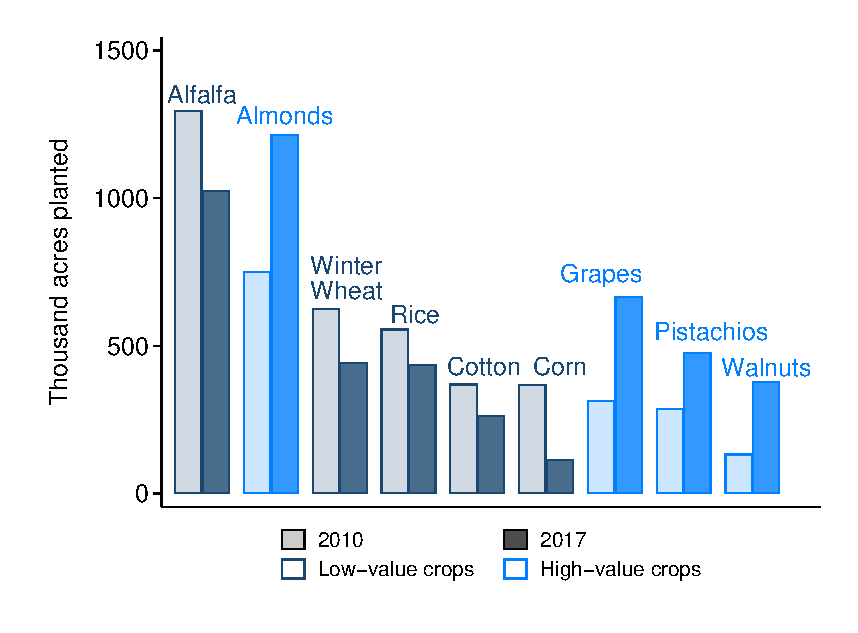
\includegraphics[width=.8\textwidth]{figures/acreage_bars2017_blue.eps}}\\
\captionsetup{width=.85\textwidth}
\caption*{\scriptsize \emph{Notes:} This figure plots the change in cropped area for nine water-intensive California crops from 2010 (light shaded) to 2017 (dark shaded): before and after the historic droughts of the mid-2010s. Crops in dark blue are relatively lower value per acre, while crops in light blue are relatively high value per acre. Acres planted measured using the USDA's Cropland Data Layer.}
\end{figure}


\begin{figure}[h!]\centering
\captionsetup{width=\textwidth}
\caption{PGE Agricultural Customers}
\label{fig:pge_ca_map}
\vspace{-2mm}
{\includegraphics[width=.8\textwidth, trim={2mm 20mm 2mm 45mm}, clip]{figures/pge_ca_map.png}}\\
\captionsetup{width=.85\textwidth}
\caption*{\footnotesize \emph{Notes:} This figure maps the locations of all agricultural service points served by PGE. Dark blue dots indicate the 11,851 service point that we can match directly to an APEP pump test. Light blue dots indicate unmatched agricultural service points. The light grey outline is the geographic boundary of PGE's service territory. }
\end{figure}

\vspace{35mm}
\begin{figure}[h!]\centering
\captionsetup{width=\textwidth}
\caption{Average marginal electricity prices}
\label{fig:marg_price_5_default_rates}
\vspace{-2mm}
{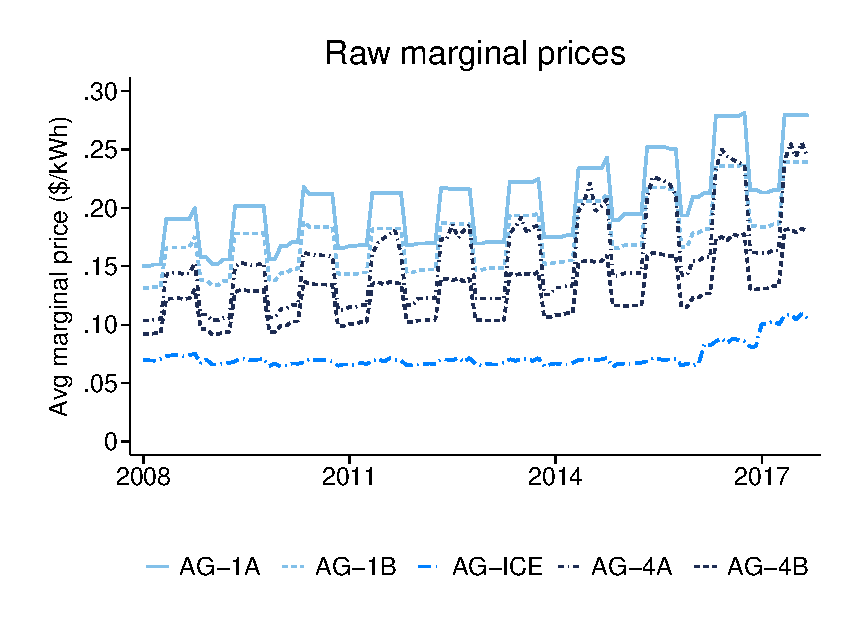
\includegraphics[width=.495\textwidth]{figures/marg_price_5_default_rates_raw.eps}}~
{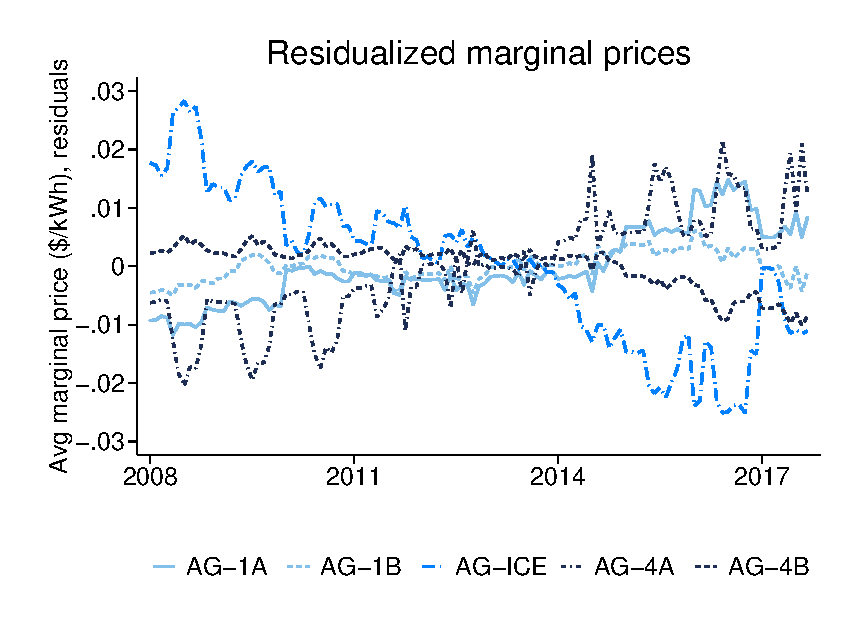
\includegraphics[width=.495\textwidth]{figures/marg_price_5_default_rates_resid.eps}}
\\
\captionsetup{width=\textwidth}
\caption*{\scriptsize \emph{Notes:} This figure plots times series of monthly average marginal electricity prices (\$/kWh) for PGE's five default agricultural tariffs. The left panel plots raw average marginal prices for each month in our estimation sample, taking unweighted averages across all hours. The right panel plots residuals of these same five time series, after partialing out tariff $\times$ month-of-year fixed effects and month-of-sample fixed effects (aligning with the fixed effects we use in estimation). AG-1A and AG-1B are non-time-varying rates (i.e.\ constant marginal price for all hours within a month), whereas AG-4A and AG-4B are time-varying rates (i.e.\ higher marginal prices during peak hours and weekdays). AG-1A and AG-4A are for small pumps ($<35$ hp), whereas AG-1B and AG-4B are for large pumps ($\ge35$ hp). AG-ICE is a time-varying rate for customers with auxiliary internal combustion engines. Marginal prices are systematically higher during summer months (May--October). Our identifying variation comes (a) strict restrictions that segment customers into categories; (b) the fact that the residualized default prices do not move in parallel; and (c) PGE's smart meter rollout, which exogenously shifted many customers from the AG-1A/1B default tariffs to the AG-4A/4B default tariffs with lower marginal prices.}
\end{figure}

\begin{figure}[t]
\begin{centering}
\caption{Histogram of pump horsepower}
\label{fig:pump_hist}
\includegraphics[width=0.7\textwidth]{Figures/pump_hist.png}
\caption*{\scriptsize \emph{Notes:} This is a histogram of measured horsepower for all 21,851 tests in our APEP pump test dataset. We observe no bunching on either side of the 35 hp cutoff that determines whether PGE classifies pumps as small or large. Bunching would be a sign that farmers optimize against PGE's tariff schedules when making pump investment decisions.}
\end{centering}
\end{figure}


\begin{figure}[t]
\begin{centering}
\caption{Hourly electricity prices and consumption}
\label{fig:hourly_consumption_vs_price}
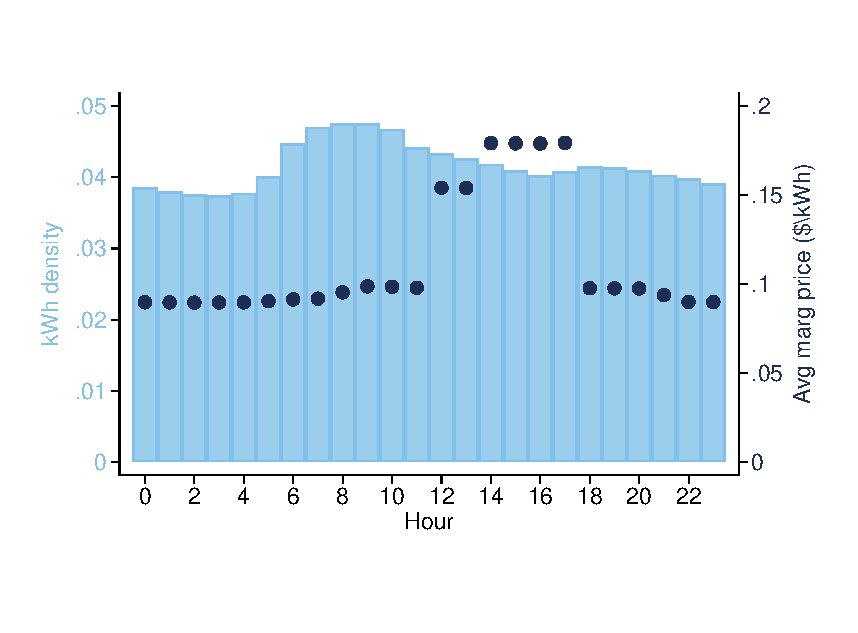
\includegraphics[trim={0 10mm 0 10mm},clip,width=.97\textwidth]{Figures/hourly_hist_prices_pooled_summer.eps}
\caption*{\scriptsize \emph{Notes:} This figure plots a histogram of electricity consumption at each hour of the day against average marginal price at each hour of the day for summer months. While average marginal prices rise substantially during the afternoon, consumption does not fall in response.}
\end{centering}
\end{figure}



\begin{figure}[t]
\begin{centering}
\caption{Modeling farm $i$'s water costs and groundwater demand response}
\label{fig:water_cost_cartoons}
\includegraphics[width=0.495\textwidth, trim={4mm 0 11mm 0mm}, clip]{Figures/water_cost_1.png}
\includegraphics[width=0.495\textwidth, trim={4mm 0 11mm 0mm}, clip]{Figures/water_cost_2.png} \\
\includegraphics[width=0.495\textwidth, trim={4mm 0 11mm 0mm}, clip]{Figures/water_cost_3.png}
\includegraphics[width=0.495\textwidth, trim={4mm 0 11mm 0mm}, clip]{Figures/water_cost_4.png}
\caption*{\scriptsize \emph{Notes:} This figure presents a stylized water price schedule for a representative farm $i$. The price schedule is nonlinear and comprises water from up to three sources: (i) a low-cost allocation of surface water from farm $i$'s irrigation district; (ii) medium-cost groundwater pumping, with costs that rise gradually in own extraction; and (iii) a high-cost backstop of open market water transactions, for which we assume farm $i$ is a price taker. For crop $k^0$ requiring $W_i(k^0)$ acre/feet of water, farm $i$'s irrigation costs $C_i\big(W_i(k^0)\big)$ are represented by the shaded region in the top-left panel. If farm $i$ experiences a pumping cost shock (due to either an electricity price increase or a groundwater depth increase), its groundwater costs shift up and its total irrigation costs increase by the shaded region $\Delta C_i\big(W_i(k^0)\big)$ in the top-right panel. The bottom panels illustrate two ways that this pumping cost shock increase translate to a reduction in farm $i$'s groundwater consumption. First, the farmer may respond to this pumping cost shock by switching from crop $k^0$ to a less water intensive crop $k^1$, as in the bottom-left panel. Second, for a large enough cost shock, the farmer may continue to grow crop $k^0$, but substitute away from groundwater using open market water purchases.
}
\end{centering}
\end{figure}

%\begin{figure}[t]
\begin{centering}
\caption{Profits in the Southern San Joaqu\'{i}n Valley under varying water prices}
\label{fig:davis_line_crossing}
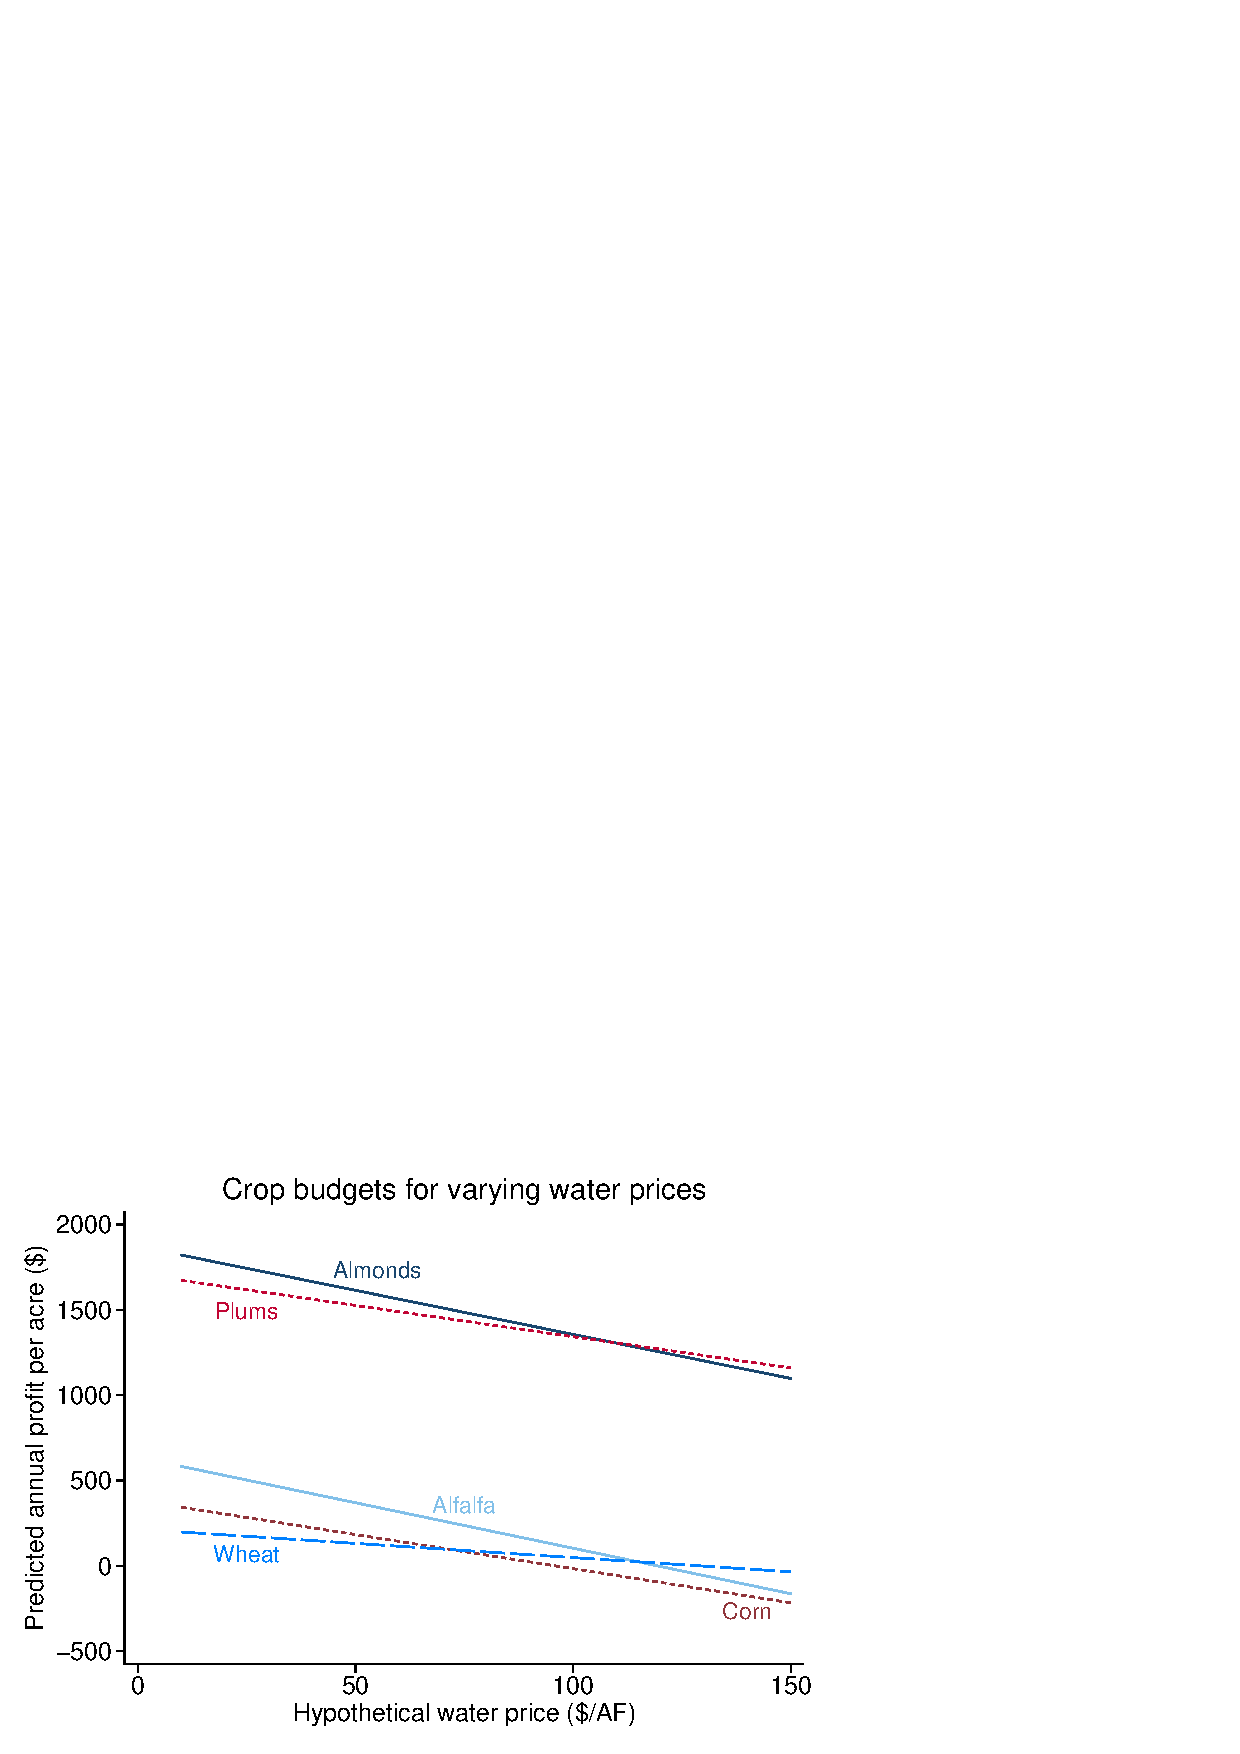
\includegraphics[width=0.7\textwidth]{Figures/davis_lines_crossing.pdf}
\caption*{\scriptsize \emph{Notes:} This figure plots annual profits per acre by crop, as reported by the UC Davis Cost Studies. We focus on five crop-specific studies in the Southern San Joaqu\'{i}n Valley, and vary the average cost of water for irrigation while holding all other assumptions constant.}
\end{centering}
\end{figure}


\begin{figure}[t]
\begin{centering}
\caption{Crop choice changes in response to a \$10 groundwater tax}
\label{fig:cf_water_tax}
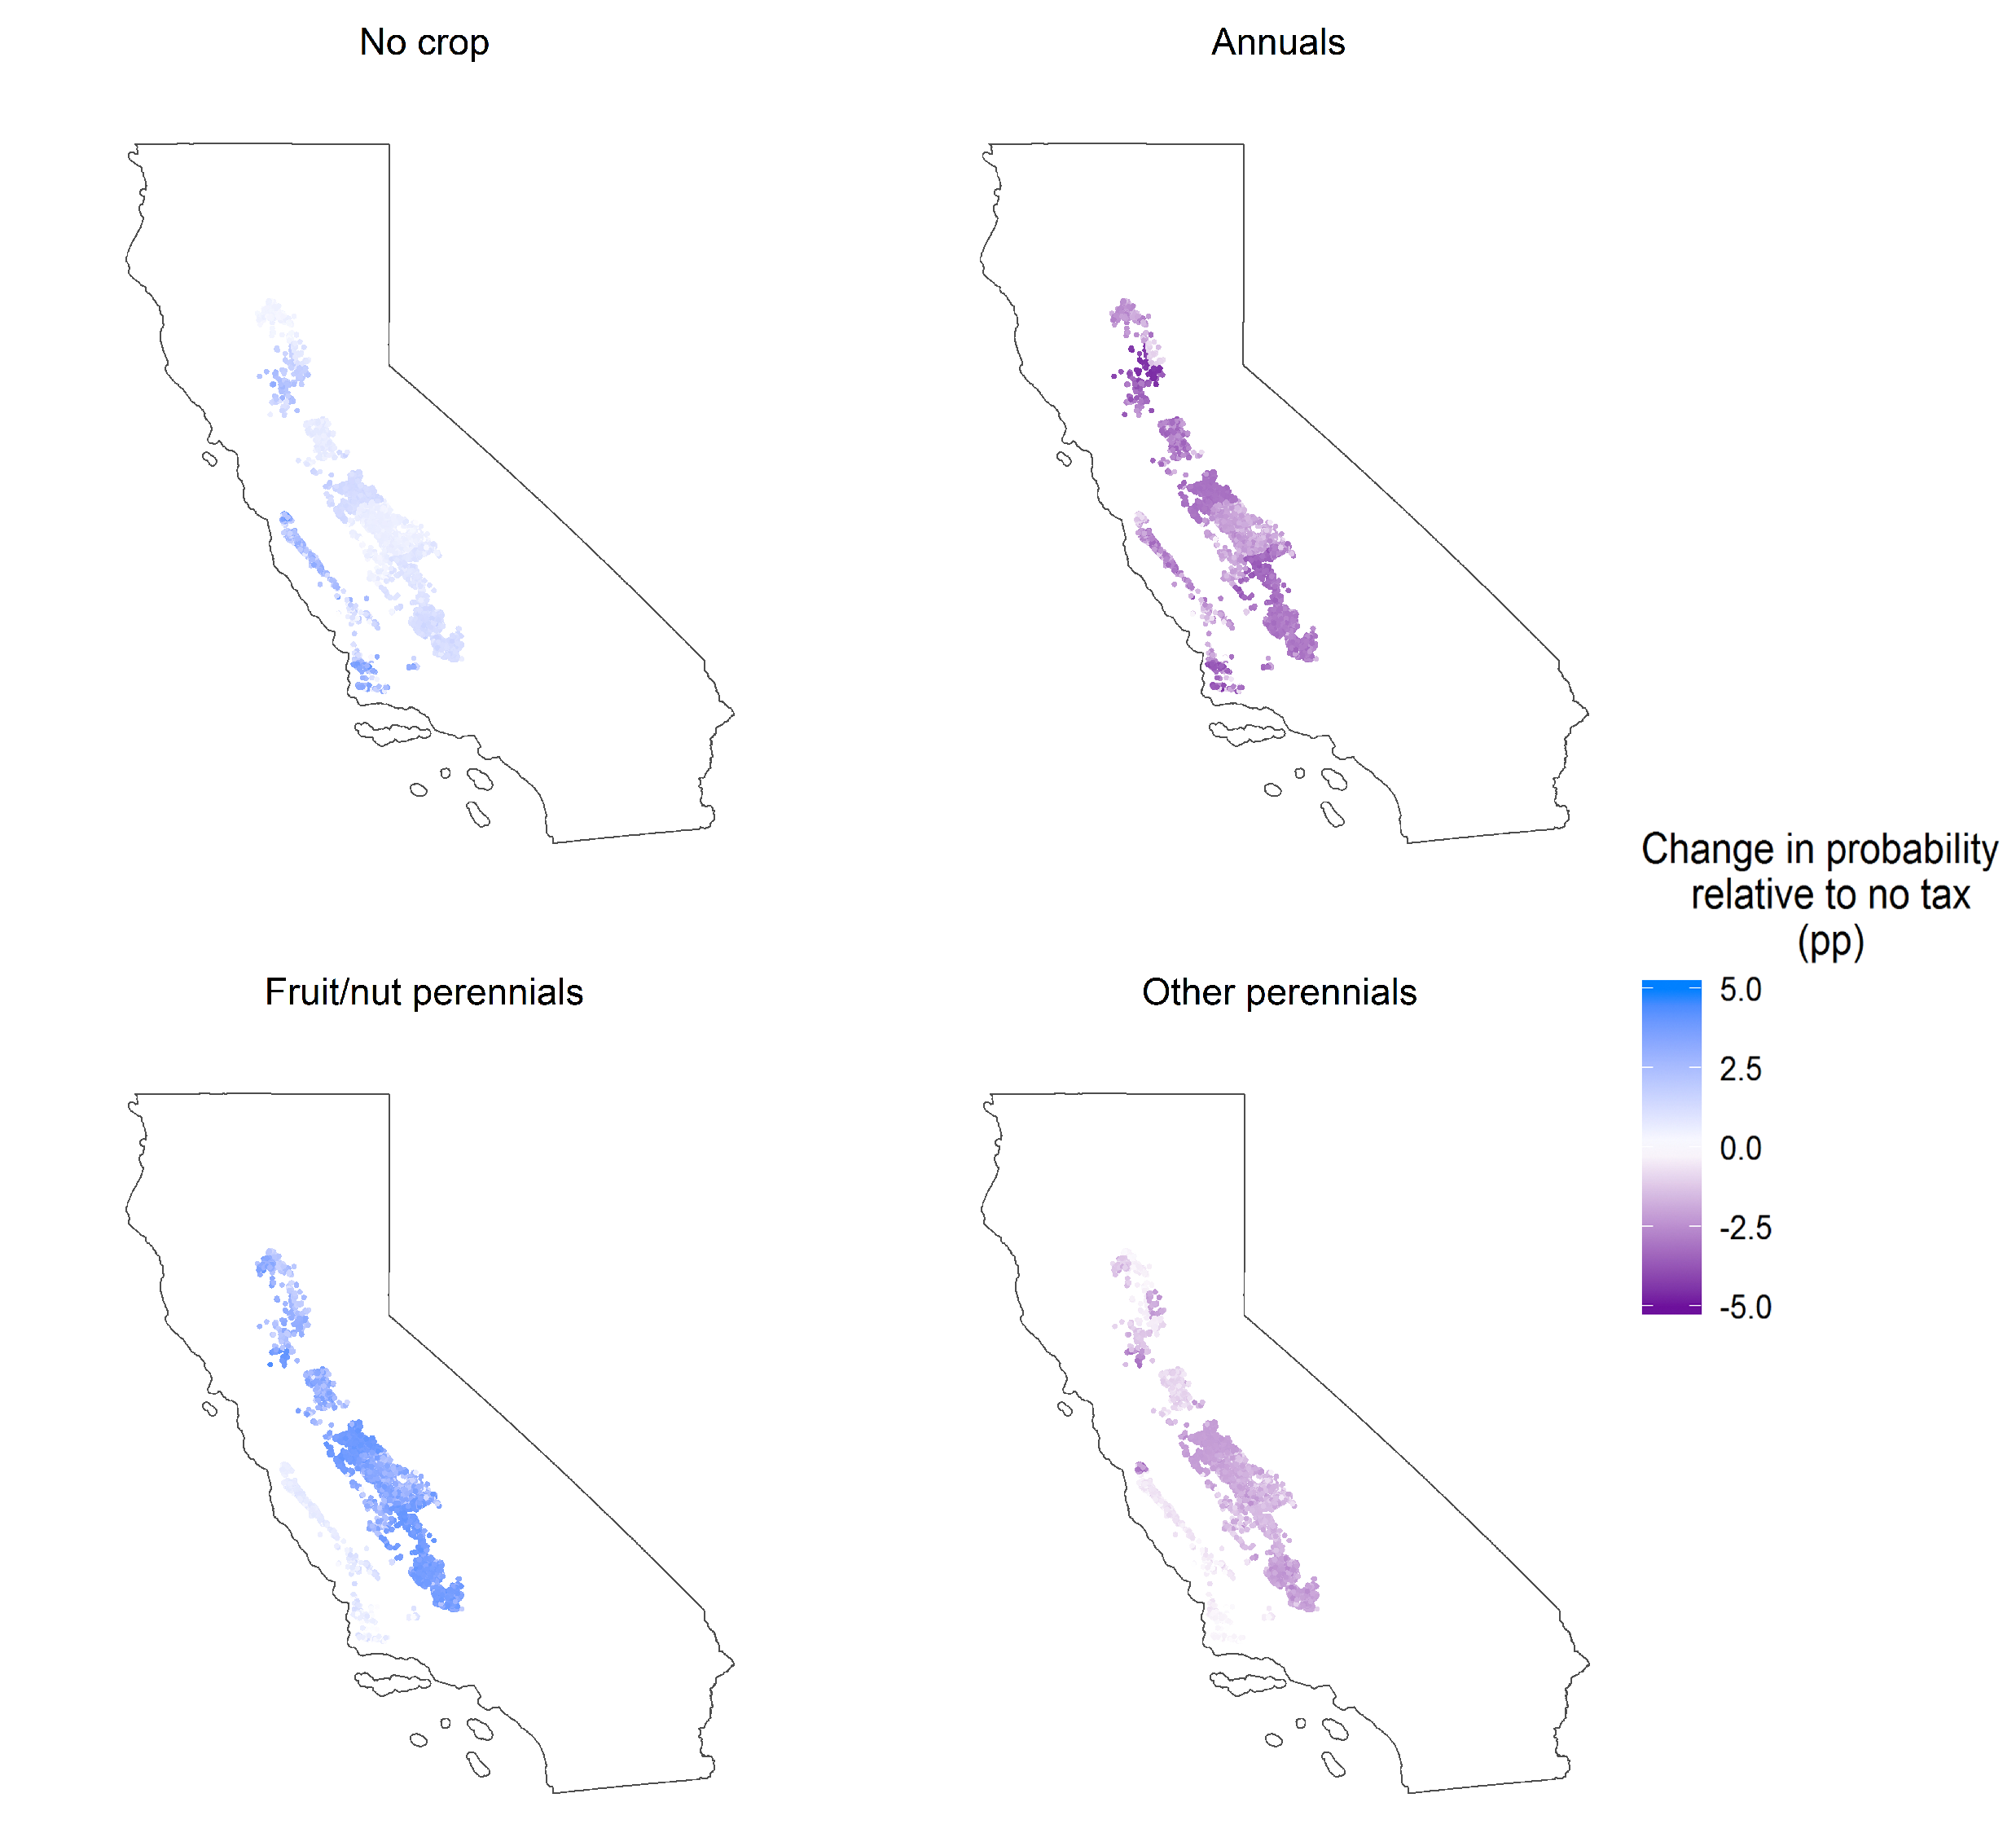
\includegraphics[width=\textwidth]{Figures/clu_prob_10tax_fullstate_combined.pdf}
\caption*{\scriptsize \emph{Notes:} This figure plots the estimated counterfactual changes in crop choice resulting from a \$10 groundwater tax, relative to no tax. Each dot is the centroid of a CLU in our sample. To generate these estimates, we first compute the average probability each CLU farms each crop type across all sample years in the no-tax baseline. We then compute similar probabilities with the groundwater price increased by \$10 per acre-foot. Finally, we subtract the no-tax baseline from the \$10 tax counterfactual to compute the change in probability of having each land type. The top left panel shows the change in fallowing. The top right panel shows the change in annual crops. The bottom left panel shows the change in fruit and nut perennials, and the bottom right shows changes in other perennials.
}
\end{centering}
\end{figure}


\FloatBarrier

\begin{table}\centering
\caption{\normalsize Summary Statistics -- Electricity Data}
\label{tab:elec_summary_stats}
\begin{tabular}{lrcrcrr}
\hline
\hline
\\ 
\vspace{-8mm}
\\
&& $\begin{matrix}\text{All Ag}\\ \text{Customers}\end{matrix}$  && $\begin{matrix}\text{Matched} \\ \text{to Pumps}\end{matrix}$ \\
[.1em]
\cline{3-5}
\\
\vspace{-7mm}
\\
Service point-month observations && 9,991,458 && 1,168,553 \\ 
[.2em]
Unique service points (SPs) && 108,172 && 11,851 \\ 
[.2em]
SPs that switch tariff categories  && 44,414 && 2,844   \\
[.2em]
SPs that switch categories (pumping capital)  && 3,454 && 561   \\
[.2em]
SPs that switch categories (smart meters)  && 43,045 && 2,553   \\
[.2em]
Share of SP-months on time-varying tariffs  && 0.702 && 0.886   \\
[.2em]
Share of SP-months on peak-day tariffs  && 0.295 && 0.152   \\
[1.4em]
Monthly electricity consumption (kWh) && 6080.9 && 12055.7   \\
 && (39783.1) && (25075.1)   \\
[.4em]
Monthly electricity consumption (kWh), summer && 8249.6 && 17589.1   \\
 && (45660.8) && (29818.5)   \\
[.4em]
Monthly electricity consumption (kWh), winter && 3849.7 && 6362.8   \\
 && (32498.8) && (17232.5)   \\
[1.4em]
Average marginal electricity price (\$/kWh) && 0.148 && 0.113   \\
 && (0.050) && (0.042)   \\
[.4em]
Average marginal electricity price (\$/kWh), summer && 0.171 && 0.130   \\
 && (0.051) && (0.044)   \\
[.4em]
Average marginal electricity price (\$/kWh), winter && 0.126 && 0.096   \\
 && (0.037) && (0.032)   \\
[1.4em]
Average monthly bill (\$, non-zero bills) && 936.66 && 1814.15   \\
 && (4662.71) && (3285.26)   \\
[.4em]
Average monthly bill (\$, non-zero bills), summer && 1398.90 && 2821.16   \\
 && (5847.34) && (4020.99)   \\
[.4em]
Average monthly bill (\$, non-zero bills), winter && 456.17 && 764.99   \\
 && (2888.86) && (1742.21)   \\
[.2em]
\hline
\end{tabular}
\captionsetup{width=\textwidth}
\caption*{\scriptsize \emph{Notes:} The left column reports summary statistics 
for the universe of agricultural electricity customers in PGE service territory, from 2008--2017.
The right column includes the subset of agricultural customers that we successfully match to a 
groundwater pump in the APEP pump test dataset---i.e., our main estimation sample.
``Pumping capital'' denotes tariff category switches driven by shifts between small pumps ($<35$ hp) and 
large pumps ($\ge 35$ hp), or adding/removing an auxiliary internal combustion engine.
Most tariff category switches were driven by PGE's smart meter rollout.
Time-varying tariffs (i.e.\ all except 1A and 1B) have higher marginal prices during peak demand hours. 
Peak-day tariffs (i.e.\ 4A, 4D, 4C, 4F, 5C, 5F) have very high marginal prices during peak
hours on the 14 highest-demand summer days.
Monthly bills include both volumetric (\$/kWh) and fixed charges (\$/kW, \$/hp, and \$/day).
Summer months are May--October.
Standard deviations of sample means in parentheses.
}
\end{table}


\begin{table}\centering
\caption{\normalsize Summary Statistics -- Pump Tests and Groundwater Consumption}
\label{tab:water_summary_stats}
\begin{tabular}{lrcrcrr}
\hline
\hline
\\ 
\vspace{-8mm}
\\
&& $\begin{matrix}\text{Matched to Pumps}\end{matrix}$ \\
[.1em]
\cline{2-3}
\\
\vspace{-7mm}
\\
Service point-month observations && 1,168,553 \\ 
[.2em]
Unique service points (SPs) && 11,851 \\ 
[1.4em]
Matched APEP points per SP && 3.45 \\ 
 && (8.80) \\
[.4em]
Operating pump efficiency (\%) && 54.46   \\
 && (11.52)   \\
[.4em]
kWh per AF conversion factor (APEP measured) && 430.30   \\
 && (254.21)   \\
[.4em]
kWh per AF conversion factor (constructed) && 346.94   \\
 && (206.03)   \\
[1.4em]
Monthly groundwater consumption (AF) && 49.0   \\
 && (151.7)   \\
[.4em]
Monthly groundwater consumption (AF), summer && 74.0   \\
 && (191.9)   \\
[.4em]
Monthly groundwater consumption (AF), winter && 23.4   \\
 && (86.6)   \\
[1.4em]
Average marginal groundwater price (\$/AF) && 39.91   \\
 && (29.63)   \\
[.4em]
Average marginal groundwater price (\$/AF), summer && 41.76   \\
 && (31.34)   \\
[.4em]
Average marginal groundwater price (\$/AF), winter && 38.01   \\
 && (27.63)   \\
[.2em]
\hline
\end{tabular}
\captionsetup{width=.93\textwidth}
\caption*{\scriptsize \emph{Notes:} These summary stats are from the merged panel of 
groundwater prices and quantities, which combines electricity data, pump test data, and groundwater data.
We observe 3.45 unique APEP pump tests for the average matched service point, although 37 percent of 
service points match to only a single APEP test.
Our constructed kWh per AF conversion factor (i.e. $\widehat{\text{kWh}\big/\text{AF}}_{it}$) uses monthly 
groundwater rasters to capture changes in (measured) kWh per AF over time, and estimation error 
compresses the right tail of distribution of measured kWh per AF. 
Monthly groundwater consumption divides electricity consumption (kWh) by $\widehat{\text{kWh}\big/\text{AF}}_{it}$. 
Grounwater prices multiply marignal electricity prices (\$/kWh) by $\widehat{\text{kWh}\big/\text{AF}}_{it}$. 
Summer months are May--October.
Standard deviations of sample means in parentheses.
}
\end{table}


\input{tables/table_elec_regs_main.tex}

\begin{table}[t!]\centering
\small
\caption{Estimated demand elasticities -- Groundwater  \label{tab:water_regs_combined}}
\vspace{-0.1cm}
\small
\begin{adjustbox}{center} 
\begin{tabular}{lcccccccc} 
\hline \hline
\vspace{-0.37cm}
\\
 & (1)  & (2)  & (3)  & (4)  & (5)  & (6) \\ 
[0.1em]
 & OLS & IV & IV & IV & IV & IV \\
\vspace{-0.37cm}
\\
\cline{2-7}
\vspace{-0.27cm}
\\
 $\log\big(P^{\text{water}}_{it}\big)$ ~ & 
 $-0.88$$^{***}$  & $-1.12$$^{***}$ & $-1.16$$^{***}$ & $-1.12$$^{***}$ & $-0.90$$^{***}$  & $-1.14$$^{***}$ \\ 
& $(0.07)$ & $(0.15)$ & $(0.17)$ & $(0.15)$ & $(0.14)$ & $(0.21)$ \\
[1.5em] 
Instrument(s): \\
[0.1em] 
~~ Default $\log\big(P^{\text{elec}}_{it}\big)$  &  & Yes & Yes  & Yes  & Yes & \\
[0.1em] 
~~ Default $\log\big(P^{\text{elec}}_{it}\big)$, lagged  & & &  &  & & Yes \\
[1.5em] 
Fixed effects: \\
[0.1em] 
~~Unit $\times$ month-of-year  & Yes  & Yes  & Yes  & Yes  & Yes  & Yes   \\ 
[0.1em] 
~~Month-of-sample  & Yes  & Yes  & Yes  & Yes  & Yes  & Yes   \\ 
[0.1em] 
~~Unit $\times$ physical capital & Yes & Yes & Yes & Yes & Yes & Yes  \\
[0.1em] 
~~Water basin $\times$ year & & &  & & Yes &   \\
[0.1em] 
~~Water district $\times$ year & & & & & Yes &  \\
[1.5em] 
Groundwater time step & Month & Month & Month & Quarter & Month & Month  \\ 
[0.1em] 
Only basins with $>1000$ SPs &  &  & Yes &  &  &   \\ 
[1.5em] 
Service point units & 10,155 & 10,155 & 9,337 & 10,155 & 10,149 & 9,922  \\ 
[0.1em] 
Months  & 117 & 117 & 117 & 117 & 117 & 105 \\ 
[0.1em] 
Observations & 0.93M & 0.93M & 0.85M & 0.93M & 0.93M & 0.82M \\ 
[0.1em] 
First stage $F$-statistic &  & 3021 & 2791 & 3198 & 4562 & 477 \\ 
[0.15em]
\hline
\end{tabular}
\end{adjustbox}
\captionsetup{width=\textwidth}
\caption*{\scriptsize \emph{Notes:} 
Each regression estimates Equation (\ref{eq:reg_water_combined}) at the service point by month level,
where the dependent variable is the inverse hyperbolic sine transformation 
of groudnwater consumed by service point $i$ in month $t$.
We estimate IV specifications via two-stage least squares, and Columns (2)--(5) instrument  
for $P^{\text{water}}_{it}$ with unit $i$'s within-category default logged electricity price. 
Column (6) instruments with the 6- and 12- month lags of this variable.
``Physical capital'' is a categorical variable for (i) small pumps, (ii) large pumps, and (iii) 
internal combustion engines, and unit $\times$ physical capital fixed effects control for shifts 
in tariff category triggered by the installation of new pumping equipment.
Water basin $\times$ year fixed effects control for broad geographic trends in groundwater depth.
Water district $\times$ year fixed effects control for annual variation in surface water allocations; 
we include a common ``no-water-district'' dummy for units not assigned to a water district, to avoid dropping them from the regression. 
Column (3) restricts the sample to only the three most common water basins (San Joaquin Valley, 
Sacramento Valley, and Salinas Valley), each of which contains over 1000 unique SPs in our estimation sample.
Column (4) uses a quarterly panel of groundwater depths to construct both $Q^{\text{water}}_{it}$ and $P^{\text{water}}_{it}$, 
rather than a monthly panel.
All regressions drop solar NEM customers, customers with bad geocodes, months with irregular electricity bills 
(e.g.\ first/last bills, bills longer/shorter than 1 month, overlapping bills for a single account),
and pumps with implausible test measurements.
Standard errors (in parentheses) are two-way clustered by service point and by month-of-sample.
Significance: *** $p < 0.01$, ** $p < 0.05$, * $p < 0.10$.
}
\end{table}


\begin{table}[t!]\centering
\small
\caption{Sensitivity to recent pump tests -- Groundwater  \label{tab:water_months_from_pump_test}}
\vspace{-0.1cm}
\small
\begin{adjustbox}{center} 
\begin{tabular}{lcccccccc} 
\hline \hline
\vspace{-0.37cm}
\\
 & (1)  & (2)  & (3)  & (4)  & (5)  \\ 
[0.1em]
 & IV & IV & IV & IV & IV \\
\vspace{-0.37cm}
\\
\cline{2-6}
\vspace{-0.27cm}
\\
 $\log\big(P^{\text{water}}_{it}\big)$ ~ & 
 $-1.10$$^{***}$  & $-1.00$$^{***}$ & $-0.92$$^{***}$ & $-1.01$$^{***}$ & $-0.90$$^{***}$ \\ 
& $(0.16)$ & $(0.17)$ & $(0.18)$ & $(0.20)$ & $(0.23)$  \\
[1.5em] 
Months away from pump test: & 60 & 48 & 36 & 24 & 12 \\
[1em] 
IV: Default $\log\big(P^{\text{elec}}_{it}\big)$  & Yes & Yes & Yes  & Yes  & Yes  \\
[1em] 
Fixed effects: \\
[0.1em] 
~~Unit $\times$ month-of-year  & Yes  & Yes  & Yes   & Yes  & Yes   \\ 
[0.1em] 
~~Month-of-sample  & Yes  & Yes  & Yes  & Yes  & Yes    \\ 
[0.1em] 
~~Unit $\times$ physical capital & Yes & Yes & Yes & Yes & Yes  \\
[1em] 
Groundwater time step & Month & Month & Month & Month & Month  \\ 
[1.5em] 
Service point units & 10,144 & 10,129 & 10,110 & 10,054 & 9,826  \\ 
[0.1em] 
Months  & 117 & 117 & 117 & 105 & 93 \\ 
[0.1em] 
Observations & 0.82M & 0.74M & 0.63M & 0.48M & 0.28M  \\ 
[0.1em] 
First stage $F$-statistic & 2803 & 2557 & 2098 & 1517 & 902  \\ 
[0.15em]
\hline
\end{tabular}
\end{adjustbox}
\captionsetup{width=\textwidth}
\caption*{\scriptsize \emph{Notes:} 
Each regression replicates our preferred specification in Column (2) from Table \ref{tab:water_regs_combined}, 
while restricting the sample to units with pump tests within $m$ months of sample month $t$. 
For example, a March 2013 observation for unit $i$ is only included in Column (3) if we observe 
a pump test for unit $i$ between March 2010 and March 2016. 
These regressions reveal that unobserved changes in pump specifications are unlikely to be systematically biasing our 
groundwater elasticity estimates. Stated differently, the mechanism underlying our estimates is unlikely to be 
unobserved changes to farmers' irrigation capital. 
See notes under Table \ref{tab:water_regs_combined} for further detail. 
Standard errors (in parentheses) are two-way clustered by service point and by month-of-sample.
Significance: *** $p < 0.01$, ** $p < 0.05$, * $p < 0.10$.
}
\end{table}


\begin{table}[t!]\centering
\small
\caption{Annual demand elasticities -- Intensive vs.\ extensive margin \label{tab:elec_water_intens_extens}}
\vspace{-0.1cm}
\small
\begin{adjustbox}{center} 
\begin{tabular}{lcccc} 
\hline \hline
\vspace{-0.37cm}
\\
 & Electricity & \multicolumn{3}{c}{Groundwater} \\
 \cmidrule(r){2-2} \cmidrule(l){3-5}
 & Overall   & Overall & Intensive & Extensive \\
 & elasticity   & elasticity & margin & margin \\
[0.1em]
 & (1)   & (2)  & (3)  & (4) \\ 
\vspace{-0.37cm}
\\
\cline{2-5}
\vspace{-0.27cm}
\\
 $\log\big(P^{\text{elec}}_{iy}\big)$ ~ & $-0.99$$^{***}$  &  &  &  \\ 
& $(0.25)$ &  &  &  \\
[0.1em] 
 $\log\big(P^{\text{water}}_{iy}\big)$ ~ &  & $-0.93$$^{***}$ & $-0.22$$^{**}$  & $-0.04$$^{***}$ \\ 
&   & $(0.24)$ & $(0.09)$ & $(0.01)$ \\
[1.5em] 
Outcome: \\
~~ $\sinh^{-1}\big(Q_{iy}\big)$ & Yes& Yes & Yes & \\
[0.1em] 
~~ $1\big[Q_{iy}>0\big]$ & & & & Yes \\
[1.5em] 
Sample restriction: \\
~~ $Q_{iy} > 0$ in all years & & & Yes & \\
[1.5em] 
Instrument: \\
[0.1em] 
~~ Default $\log\big(P^{\text{elec}}_{iy}\big)$  & Yes   & Yes  & Yes & Yes \\
[1.5em] 
Fixed effects: \\
[0.1em] 
~~Unit $\times$ physical capital & Yes & Yes & Yes & Yes  \\
[0.1em] 
~~Water basin $\times$ year & Yes & Yes & Yes & Yes \\
[0.1em] 
~~Water district $\times$ year &  Yes & Yes & Yes & Yes \\
[1.5em] 
Service point units & 10,113  & 9,058 & 4,270 & 9,058  \\ 
[0.1em] 
County $\times$ years  & 270 & 268 & 236 & 268 \\ 
[0.1em] 
Observations & 58.2K  & 51.8K & 25.0K & 51.8K \\ 
[0.1em] 
First stage $F$-statistic & 2165  & 2425 & 1092 & 2425 \\ 
[0.15em]
\hline
\end{tabular}
\end{adjustbox}
\captionsetup{width=\textwidth}
\caption*{\scriptsize \emph{Notes:} Each regression estimates Equation (\ref{eq:reg_elec_annual}) or Equation (\ref{eq:reg_water_annual}) at the service point by year level.
Column (1) reports results for electricity consumption, and Columns (2)--(4) report results for groundwater consumption.
Columns (1) and (2) report annual demand elasticities for electricity and water, respectively. These results are analogous to the monthly demand elasticities reported 
in Column (4) of Table \ref{tab:elec_regs_main} and in Column (5) of Table \ref{tab:water_regs_combined}, respectively.
Column (3) reports an analogous demand elasticity for the subset of service points that consume water in every year of our sample.
Column (4) reports the semi-elasticity for the extensive margin by replacing the outcome variable with a binary indicator water consumption.
We estimate these regressions using two-stage least squares, instrumenting with unit $i$'s within-category default logged electricity price in year $y$.
``Physical capital'' is a categorical variable for (i) small pumps, (ii) large pumps, and (iii) internal combustion engines, and unit $\times$
physical capital fixed effects control for shifts in tariff category triggered by the installation of new pumping equipment.
Water basin $\times$ year fixed effects control for broad geographic trends in groundwater depth.
Water district $\times$ year fixed effects control for annual variation in surface water allocations.
All regressions drop solar NEM customers, customers with bad geocodes, years with irregular electricity bills
(e.g.\ first/last bills, bills longer/shorter than 1 month, overlapping bills for a single account), and incomplete years.
Groundwater regressions use a monthly time interval to assign rasterized groundwater levels.
Standard errors (in parentheses) are two-way clustered by service point and by county-year.
Significance: *** $p < 0.01$, ** $p < 0.05$, * $p < 0.10$.
}
\end{table}


\begin{table}[t!]\centering
\small
\caption{Crop switching estimates -- Discrete choice model \label{tab:probit_results}}
\vspace{-0.1cm}
\small
\begin{adjustbox}{center} 
\begin{tabular}{lcc} 
\hline \hline
\vspace{-0.37cm}
\\
 & Marginal effect & Semi-elasticity \\
\vspace{-0.37cm}
\\
\cline{2-3}
\vspace{-0.27cm}
\\
Annuals & $-0.252$$^{***}$ & $-0.088$$^{***}$ \\ 
& $(0.042)$ & $(0.013)$ \\ 
[0.1em]
Fruit and nut perennials & $0.307$$^{***}$ & $0.104$$^{***}$ \\ 
& $(0.055)$ & $(0.020)$ \\ 
[0.1em]
Other perennials & $-0.162$$^{***}$ & $-0.053$$^{***}$ \\ 
& $(0.034)$ & $(0.010)$ \\ 
[0.1em]
Fallow & $0.107$$^{***}$ & $0.038$$^{***}$ \\ 
& $(0.033)$ & $(0.013)$ \\ 
[1.5em]
Instrument: \\ 
[0.1em] 
~~Default $\log(P^{\text{elec}}_{iy})$ & \multicolumn{2}{c}{Yes} \\ 
Fixed effects: \\ 
[0.1em] 
~~County $\times$ year $\times$ crop type & \multicolumn{2}{c}{Yes} \\ 
[1.5em] 
Common land units & \multicolumn{2}{c}{7,380} \\ 
[0.1em] 
Observations & \multicolumn{2}{c}{36,799} \\ 
[0.1em] 
First stage $\chi^2$-statistic & \multicolumn{2}{c}{1134} \\ 
[0.15em]
\hline
\end{tabular}
\end{adjustbox}
\captionsetup{width=\textwidth}
\caption*{\scriptsize \emph{Notes:} We estimate the discrete choice model of Equation (\ref{eq:discrete_choice}) using IV probit, instrumenting for groundwater price with the default within-category electricity price. 
We include county-by-year-by-crop-type fixed effects to flexibly estimate profit excluding the cost of groundwater pumping.
The left column presents the average marginal effects of groundwater price on crop type choice probabilities.
The right column reports the average semi-elasticities for each crop type choice probability with respect to the groundwater price.
Each value is calculated for every observation in our analysis, and then we take the mean over all observations to yield these average values. 
Standard errors (in parentheses) are clustered at the common land unit (CLU).
Significance: *** $p < 0.01$, ** $p < 0.05$, * $p < 0.10$.
}
\end{table}


\begin{table}[t!]\centering
\small
\caption{Counterfactual groundwater taxes \label{tab:sim_acres}}
\vspace{-0.1cm}
\small
\begin{adjustbox}{center} 
\begin{tabular}{lcccc} 
\hline \hline
\vspace{-0.37cm}
\\
 & No tax & \$5 tax & \$10 tax & \$15 tax \\
\vspace{-0.37cm}
\\
\cline{2-5}
\vspace{-0.27cm}
\\
Simulated acreage (thousands of acres) & & & & \\ 
~~Annuals & $61.74$ & $57.85$ & $54.09$ & $50.45$ \\ 
[0.1em]
~~Fruit and nut perennials & $147.30$ & $151.69$ & $155.93$ & $160.03$ \\ 
[0.1em]
~~Other perennials & $34.24$ & $31.94$ & $29.71$ & $27.57$ \\ 
[0.1em]
~~Fallow & $71.60$ & $73.40$ & $75.15$ & $76.83$ \\ 
[0.5em]
~~Total reallocation & & $12.37$ & $24.35$ & $35.92$ \\ 
~~Total reallocation (percent) & & $(3.9\%)$ & $(7.7\%)$ & $(11.4\%)$ \\ 
[0.5em]
Change in groundwater consumption (percent) & & $-13.7\%$ & $-27.3\%$ & $-41.0\%$ \\ 
[0.15em]
\hline
\end{tabular}
\end{adjustbox}
\captionsetup{width=\textwidth}
\caption*{\scriptsize \emph{Notes:} This table reports the results of adding counterfactual taxes on groundwater to the observed electricity prices in our sample.
To simulate the impacts of a groundwater tax, we first calculate the choice probability of each crop type (annuals, fruit/nut perennials, other perennials, and no crop) for each CLU in our sample over our time series.
This baseline allocation is represented in the first column, labeled ``No tax.'' The sample average marginal price is \$41.00 per acre-foot. 
In the subsequent columns, we take each CLU's average annual marginal price and add the reported tax level to it. We then calculate choice probabilities for this counterfactual groundwater price.
The first four rows correspond to the four crop types in our analysis, and the table displays the total acreage in our sample that we predict would be cropped in each crop type under each of the tax levels.
The fifth row reports the total acreage of cropland that is reallocated to a different crop type due to the groundwater tax, as compared to no tax.
The sixth row displays the total percent change in land use for each tax level, as compared to no tax.
These reallocations estimates are based on the 314,884 acres of agricultural land matched to our sample.
The final row reports the estimated change in groundwater consumption, using our groundwater elasticity estimate of $-1.12$, for each tax level. 
}
\end{table}


\end{document}
